\chapter{Literature study}
\label{chap:rel_work}
In order to correctly implement a solution, we need to understand the fundamentals.
These consist of 2 research fields: \gls{HPE} and \gls{NST}.
The former will be used to detect poses in the art collections, but not before the latter has tried to make an improvement.
Following will be an overview of the available research in these domains.
Discussing what the goals of them are, how they achieve it, what their challenges are and their limitations.

\section{Human Pose estimation}
\label{sec:hpe}

\gls{HPE} aims to detect human features from input data such as images and videos.
It's an elementary part of computer vision with many applications among which are human action recognition (sign language), human tracking (surveillance), and human-computer interaction (video games).
This is an extensively researched area with a diverse range of different techniques.
This chapter will try to give an overview of all the many challenges and proposed solutions.
The focus will be on deep learning models, which have surpassed classical solutions significantly.
Specifically, around 2D monocular \gls{HPE} eg., \cite{Munea2020}\cite{Zheng2012}\cite{Liu2104}\cite{chen2022}.

The human body has a high degree-of-freedom due to all the limbs, self-similar parts and body types, which may cause self-occlusion or rare/complex poses.
The variations in configuration are made even larger due to clothing, lighting, foreground occlusion, as well as viewing angles and truncation, among others, as shown in fig. \ref{fig:hpe_problem_complexity}.
This makes \gls{HPE} one of the most difficult tasks in computer vision \cite{jain2014}\cite{Chen2000}.

\subsection{Representation}
\label{section:representation}

An important factor in \gls{HPE} is how the pose will be represented.
Depending on the needs of the problem you can have a skeleton-base, contour-base, or volume-base solution \cite{Chen2000}\ref{fig:pose_representation}.

\subsubsection{Skeleton-based model}
The skeleton is build of a tree-structured set of keypoints that represent the joints of the human body.
These can be explicitly described by their coordinates in 2D or 3D space \cite{Toshev2014}.
More suitable for a \gls{CNN} however is a heatmap which constructs a 2D Gaussian kernel around a keypoint \cite{Liu2104}\cite{SWARH}.
They are easily implemented and became the dominant representation.
While the skeleton-based model is a compact and flexible representation it suffers in this aspect by not being able to hold texture or shape information \cite{Zheng2012}.

\subsubsection{Contour representation}
To capture the shape of the body parts, contour representation uses rectangles to estimate the body contours.
These methods include cardboard models \cite{Ju96} and \gls{ASMs} \cite{COOTES95} and were mainly in use in earlier \gls{HPE} methods \cite{Chen2000}.

\subsubsection{Volume representation}
Volumetric geometric shapes can also be used as a method of representation.
Earlier methods used simple shapes like cylinders, conics, and other shapes \cite{Sidenbladh2000}.
Volume representation is a 3D mesh that represents the human body.
The most used model is \gls{SMPL}, which includes natural pose-dependent deformations imitating soft-tissue dynamics \cite{Loper2015}.  
\\
\\
For the purpose of our research, a simple model is the only thing we need.
We only need to be aware of the most essential joints to label a pose.
This makes the skeleton-based model the ideal representation to work with and will be the focus of further study.

\subsection{Datasets}
There are several publicly available datasets.
There are some that are outdated and we will leave those out, focusing only on datasets used for deep learning.

\textbf{\gls{LSP} Dataset \cite{Johnson2010}} contains 2,000 images found on Flickr using 8 different tags looking for sport activities (athletics, badminton, baseball, gymnastics, parkour, soccer, tennis, and volleyball).
Each person has 14 keypoints.
An extended version was later introduced \cite{Johnson2011}, now consisting of 10,000 images. 
For this set they only focused on the more challenging tags (parkour, gymnastics, and athletics).

\textbf{\gls{MPII} Human Pose Dataset \cite{Andriluka2014}} contains 24,290 images with 40,522 labeled people.
They were extracted from YouTube videos found by querying for physical activities.
Each person has 16 keypoints and also includes occlusion labels.

\textbf{\gls{COCO} Dataset \cite{Lin2014}} is a large-scale dataset for a wide range of computer vision algorithms.
For \gls{HPE}, the set contains more than 200,000 images in which 250,000 persons are annotated.
Each person has 17 keypoints, a bounding-box and visibility labels.
This dataset has become the most popular for benchmarking.

\textbf{\gls{FLIC} Dataset \cite{Sap2013}} contains 5,003 images extracted from Hollywood movies.
They ran a person detector which collected 20,000 images from 30 movies.
Occluded and difficult poses were then removed leaving only 5,000 images to be annotated.
Only the upper body received 10 keypoints.

\textbf{\gls{AIC-HKD} Dataset \cite{Sap2013}} contains 300,000 images found using Internet search engines.
In these, over 700,000 humans are annotated.
Each person has 14 keypoints, a bounding-box, as well as visibility and left/right labels.

\textbf{CrowdPose Dataset \cite{Li2018}} puts an emphasis on crowded images.
30,000 images from \gls{MPII}, gls{COCO} and gls{AIC-HKD} were measured with a Crowd Index, which evaluates the crowdedness.
Finally, 20,000 images are selected and 80,000 persons annotated.
Each person has 14 keypoints and a full-body bounding box.


\subsection{Discriminative Methods and Generative Methods}
Before deep learning became prominent in \gls{HPE} there were already a number of different methods in use.
Some of these methods are compatible with the deep learning methods and were thus adopted.
An early distinction is between generative and discriminative methods.

\subsubsection{Generative Model}
A generative method will work with prior beliefs about the pose.
More information about this can be found in the section about representation \ref{section:representation}.
It will project the pose on the image and verify it with the image data.
If they don't comply, the pose is adjusted using the descent direction found by minimizing an error function \cite{Pons-Moll2011}.

\subsubsection{Discriminative Model}
Discriminative methods on the other hand, try to map the pose on the image data with learned models.
There are several methods in this category, among which are the deep learning-based methods.
The deep-learning methods are further categorized by the following sections.

\subsection{Single-Person Methods}
Single-person pose estimation will try to evaluate only one pose from an image.
There are 2 major methods that are in use: regression methods and detection-based methods.

\subsubsection{Regression-based Methods}
The regression-based methods learn a network that maps all the body keypoints to the image-data directly as show in \ref{fig:single_pose_estimation_regression_methods}.

The first successful deep learning model came from Toshev and Svegedy \cite{Toshev2014} and is considered the switch in paradigm from classic approaches to deep learning \gls{HPE}.
Toshev et al. uses a 7-layered model with 5 convolution layers and 2 fully-connected layers for the pose regressor, based on AlexNet for its simple but effective architecture \cite{AlexNet}.
They then cascade the resulting found keypoints of this model to itself where it refines it using the area around the keypoints.
While the network is the same, the different stages will have different learned parameters.
With every stage the found keypoints become more accurate.

Carreira et al. \cite{CarreiraAFM15} introduce an Iterative Error Feedback which is a self-correcting model using top-down feedback.
Using the image-data and a starting pose modeled as a heatmap, the model, based on GoogLeNet \cite{googlenet}, will predict an error for each keypoint.
The pose is then corrected based on the error and fed back into the model as a heatmap with the image.
With each iteration it converges towards the solution instead of making the prediction in one go.
Regression-based methods map the keypoints directly on the image, making it a non-linear problem.
This will cause less robust generalization \cite{Liu2104}.

\subsubsection{Heatmap/Detection-based Methods}
The detection-based methods will first estimate the individual body parts using heatmaps, which leads to an easier optimization and a more robust generalization \cite{chen2022}.
Most of the latest \gls{HPE} methods use heatmaps because of this.
After the joints are found they are then assembled to fit a human skeleton.
This process is shown in \ref{fig:single_pose_estimation_heatmap-based_methods}.

Tompson et al. \cite{TompsonJLB14} proposed a hybrid architecture where the detection of body parts is handled by a \gls{CNN} and a Spatial-Model to bring those together.
The first step produces many false-positives and these are removed in the second step by restricting joint inter-connectivity to enforce correct anatomy.
They build on this in \cite{Tompson2015}, where they used a cascade to refine predictions.

A fundamental work written by Wei et al. \cite{Wei2016} combines convolution networks with Pose Machines \cite{Ramakrishna2014}.
Pose Machines is an iterative architecture which consists of 2 models: the first is used for stage 1 where it extracts potential heatmaps for the joints.
The second model is used for subsequent stages where the result of the previous stage is fed in together with the results of its own convolution network on the input image. 
This gradually refines the predictions for the joints and their positioning.
\ref{fig:convolutional_pose_machines} shows this process.

Another influential work was being written at the same time by Newell et al. \cite{Newell2016}.
Similar to \gls{CPMs}, this is also an iterative architecture.
They suggest what they call a "stacked hourglass" network, where "hourglass" modules are repeated \ref{fig:single_pose_estimation_stacked_hourglass}.
In an "hourglass" module, first, the features are downsampled and afterwards upsampled again \ref{fig:single_pose_estimation_hourglass_module}.
This network captures different spatial relationships between joints at different resolutions.
Several other works \cite{Yang2017}\cite{Yu2017}\cite{Chou17} have since improved on the network design.

Both these use intermediate supervision to tackle the problem of vanishing gradients.
This still doesn't build a deep sub-network for feature extraction which limits the estimations.
This has become less of a problem with the emergence of \gls{ResNet}\cite{He2015} which allows better back-propagation at deeper levels through shortcuts.

A more recent work by Sun et al. \cite{Sun2019} maintains the high-resolution representations instead of working the high-resolution from the low-to-high sub-network.
After a first high-resolution sub-network, it gradually adds high-to-low sub-networks in parallel to predict multi-resolution features.
Before each branch, they apply multi-scale fusion, which joins the predicted features from each scale on each scale.
Both are shown in \ref{fig:HRNet}.
This network has proven very effective and inspired several variations \cite{Cheng2019}\cite{Yu2021}\cite{Yuan2021}.

With the emergence of neural networks also came \glspl{GAN} \cite{Goodfellow2014}, which proved useful for \gls{HPE}.
They are employed to improve constraints of joint inter-connectivity and infer occluded body parts.

Chen et al. \cite{Chen2017} propose a structure-aware convolution network using a stacked hourglass as generator which generates heatmaps for each joint.
They use 2 discriminators, one to discriminate between low- and high-confidence predictions, another for real and fake poses.
The network is designed as a \gls{cGAN} \cite{Mirza2014}, which allows it to generate pose heatmaps as well as occlusion heatmaps.

A more classic \gls{GAN} is used by Chou et al. \cite{Chou2017}, where they use a stacked hourglass network for both the generator as the discriminator.
The generator predicts the heatmaps for each joint and the discriminator distinguished between the real and fake ones.

\subsection{Multi-Person Methods}
With multi-person methods comes an extra layer of difficulty: they need to be able to detect each person separately.
To solve this problem multi-person methods propose several solutions. 
The 2 most popular are top-down and bottom-up methods.

\subsubsection{Top-Down Methods}
This method will first try to detect all persons in the image with a human detector.
Each person is cropped by the bounding box and a single-person estimator predicts a pose for each person.

Occlusion and truncation are a regular occurrence in multi-person scenes and inevitable problem.
One of the early multi-person models, by Iqbal et al. \cite{Iqbal2016}, works towards creating a robust model against occlusion.
It uses Faster RCCN \cite{Ren2015} to detect the human boundaries.
After which, it applies integer linear programming for each person's fully connected graph.
This technique is similar to \cite{Pishchulin2015}, but instead of working on all globally found joints it only considers local joints.
It can also handle any kind of occlusion or truncation.

The use of a human detector comes with its own sort of problems.
Fang et al. \cite{Fang2016}, with \gls{RPME}, try to remedy these with 2 components:
They try to tackle inaccurate bounding boxes with Symmetric Spatial Transformer Network, redundant detections with Parametric Pose Non-Maximum-Suppresion.
They also propose a 3rd component, Pose-Guided Proposals Generator, which can augment training samples.

Papandreou et al. \cite{Papandreou2017} use a 2 stage pipeline.
In the first stage, they employ the Faster RCNN detector \cite{Ren2015}.
In the second stage, they estimate the pose in each found bounding box using their own network.
It predicts heatmaps using a fully convolutional \gls{ResNet} and use their own novel aggregation procedure.
Afterwards, they do post-processing using keypoint-based \gls{NMS} a method of their own making.

A continuous effort is taken by Chen et al. \cite{Chen2017} to deal with occlusion and truncation.
They suggest a 2 stage architecture, a \gls{CPN} as seen in \ref{fig:cascade_pyramid_network},
where first the "simple" keypoints are captured with GlobalNet, a feature pyramid network based on \cite{Lin2016},
and the "hard" keypoints are handled by their RefineNet, based on the upsampling and concatenating of HyperNet \cite{Kong2016} and using an adapted stacked hourglass.
They achieved great results and several others improved on their work \cite{Su2019}\cite{Li2019}.

In more recent research, a new method was become more powerful than \glspl{CNN}.
The Transformer \cite{Vaswani2017}, based on attention mechanisms which are used to optimize recurrent networks \cite{Kim2017}, eliminates the use of recurrent layers, keeping only the attention mechanisms.
Yang et al. \cite{Yang2020} use this architecture because allows for better understanding of the spatial dependencies and learns at a higher rate.

\subsubsection{Bottom-Up Methods}
A different approach is taken with bottom-up methods.
They first locate all joints in the image and then assemble them in potential humans.

DeepCut by Pishchulin et al. \cite{Pishchulin2015}, one of the first multi-person models using \glspl{CNN}.
Using Fast R-CNN \cite{Ren2015}, it detects the body parts and labels each.
With the joints found, it then uses \gls{ILP} to assemble them.
This method is very computationally expensive; NP-hard.
Insafutdinov et al. \cite{Insafutdinov2016} therefor introduce a stronger part detector and better optimization strategy with DeeperCut.

\gls{CPMs} make a return with OpenPose by Cao et al. \cite{Cao2018}, they're used to predict the joints with heatmaps and \glspl{PAFs}.
A part affinity field also encodes the position and orientation of the limb which makes the assembly of joints into different poses possible.
They can achieve real-time results with this method, and several others have improved on their design \cite{Zhu2017}\cite{Hidalgo2019}\cite{Li2019}.
The high performance is only applicable to high-resolution images.
Low-resolution images or images with occlusions perform poorly.

Kreiss et al. \cite{Kreiss2019} continue on the idea of fields and introduce the \gls{PIF} and \gls{PAF}.
First, they predict the location of the different joints with \gls{PIF}.
Afterwards, they use \gls{PAF} to find the inter-joint relationships.
They are able to outperform any previous OpenPose-based proposals on low-resolution and occlusions.

Newell et al. \cite{Newell2016-2} introduce a new method called associative embedding for supervising \glspl{CNN} both detection and grouping.
This is a single-stage architecture as opposed to the two-staged architectures previously discussed.
They make use of the stacked hourglass network from \cite{Newell2016} with some small modifications.

Continuing on the idea of associative embedding, Cheng et al. \cite{Cheng2019} use HRNet \cite{Sun2019} as backbone for their HigherHRNet.
Their method focuses on the scale-variance problem; a problem which hasn't been studied much, so it can localize keypoints for small persons better.
Lou et al. \cite{Lou2020} introduce \gls{SAHR} and \gls{WAHR} to the scale-variance problem.
\gls{SAHR} adaptively adjusts the standard deviation of each heatmap corresponding with the scale of the person.
\gls{WAHR} rebalances the foreground and background samples, so \gls{SAHR} can work to its fullest extent.

\subsubsection{Summary}
An important challenge for \gls{HPE} is making predictions in scenes with hight occlusions.
Top-down models achieve state-of-the art performance in almost all benchmark datasets \cite{Chen2000}.
Top-down models has difficulty with overlapping bodies and human detectors might fail finding humans there.
To the same extent, bottom-up models will have greater inaccuracy with grouping in occluded scenes.
Computationally, the top-down model's speed is limited by the number of people found.
The higher efficiency of bottom-up models, make them more suitable for real-time applications.

\begin{figure}
	\centering
	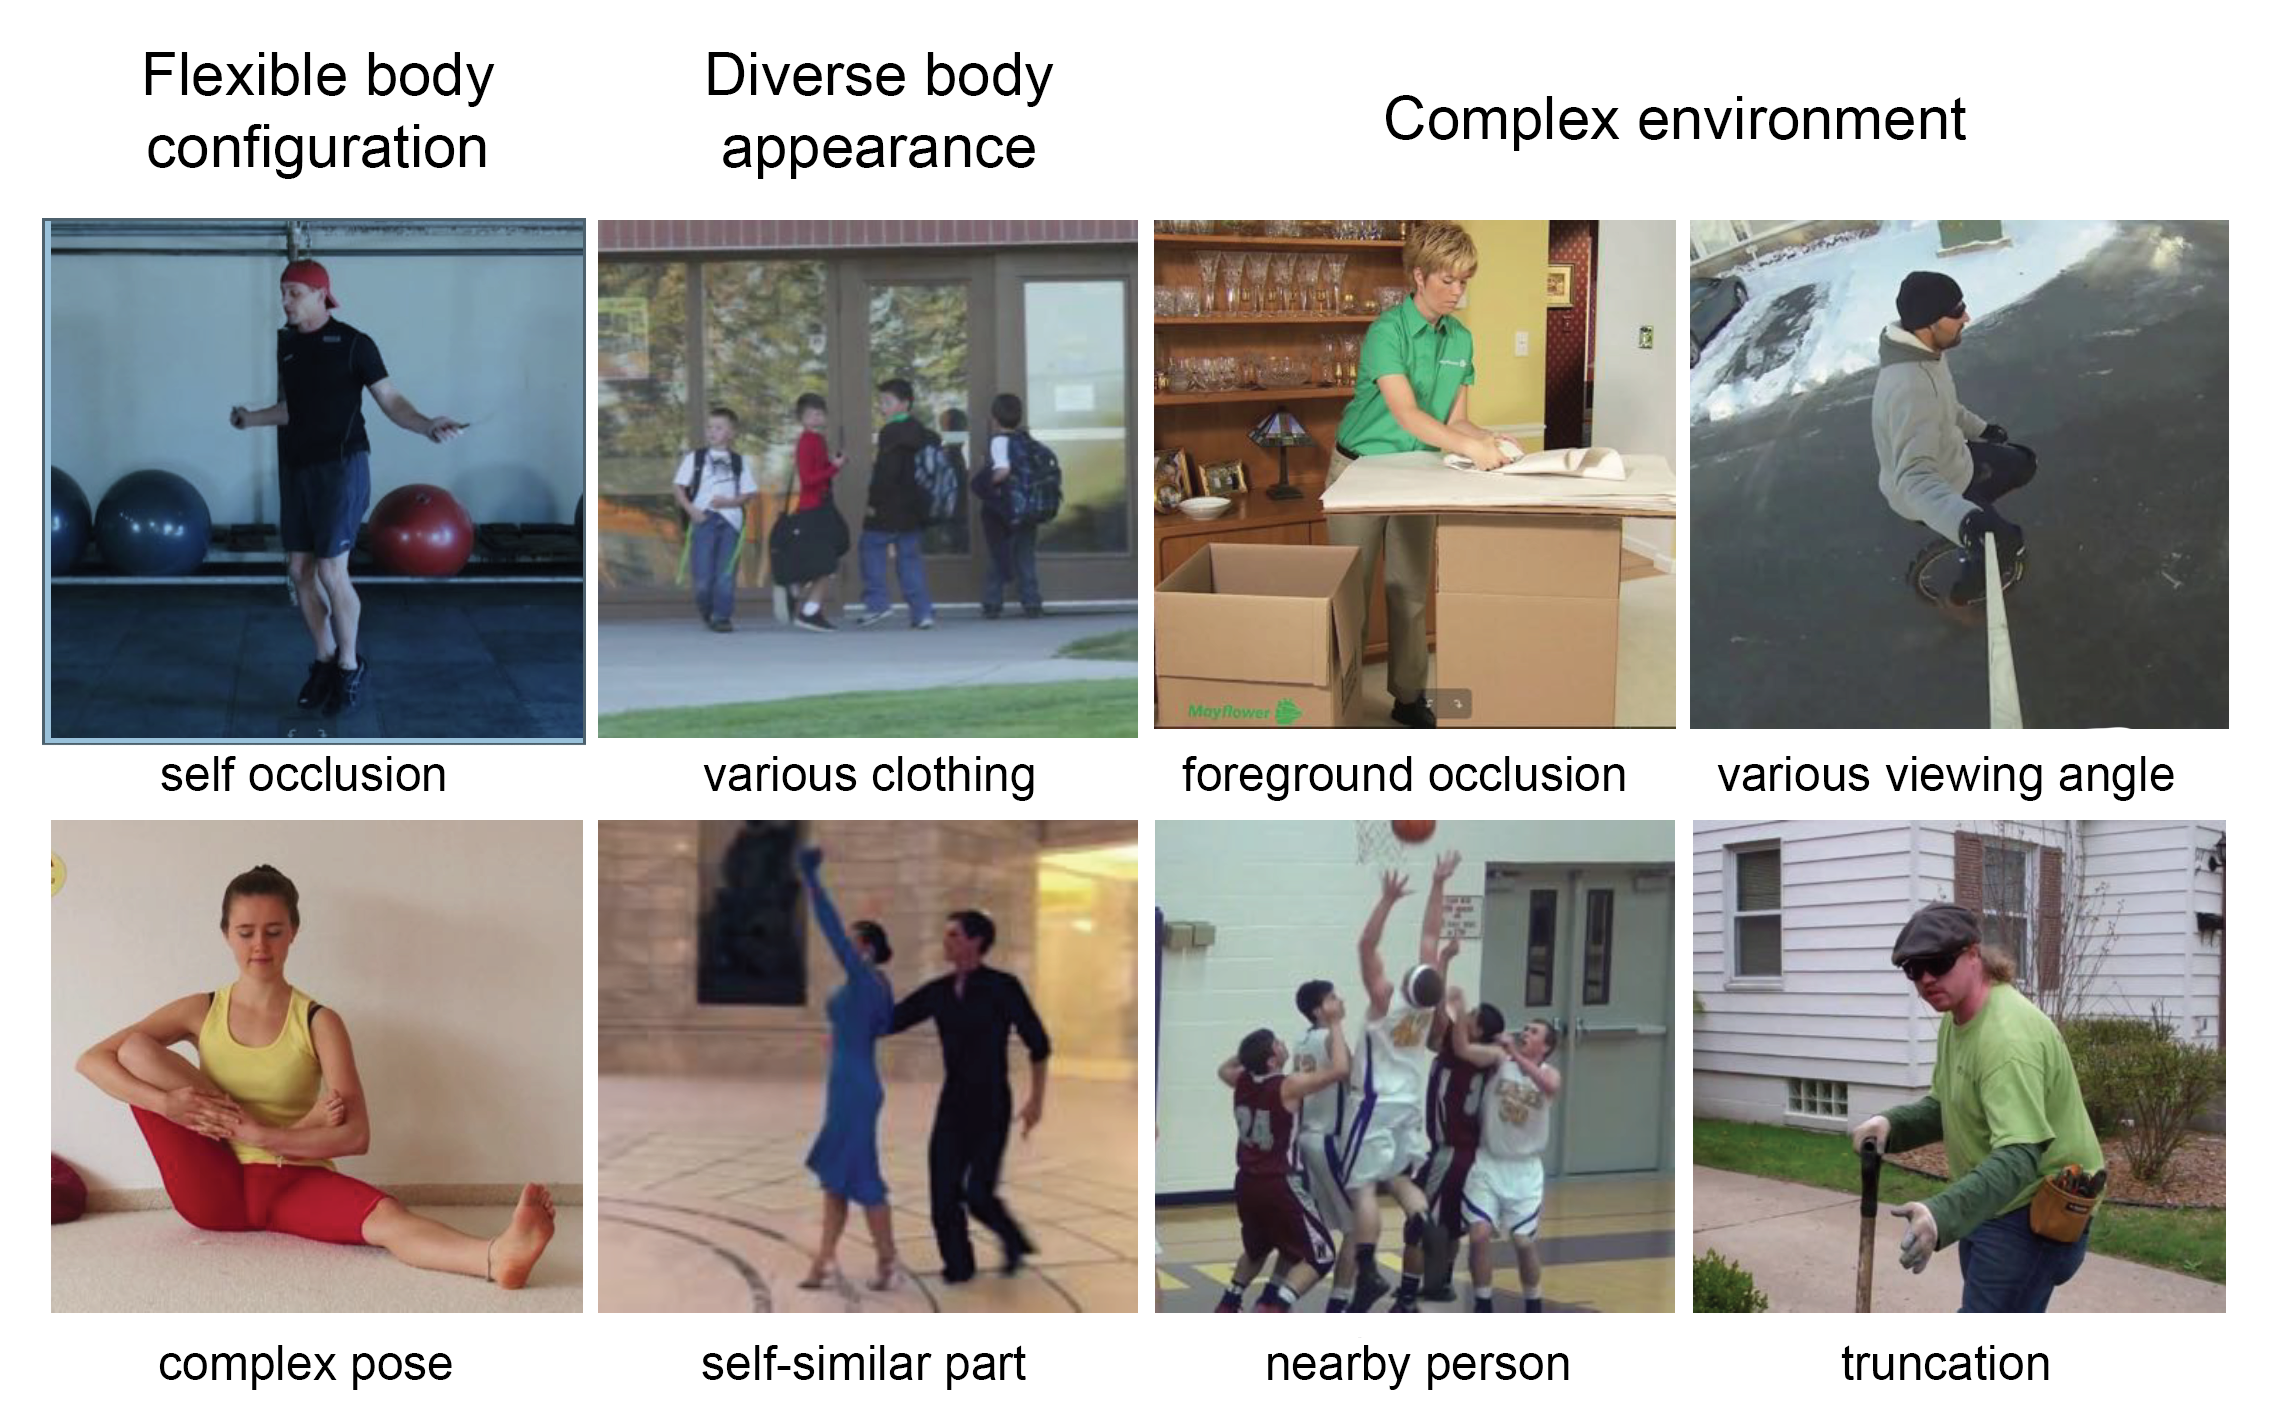
\includegraphics[width=1\textwidth]{hpe_problem_complexity}
	\caption{The various challenges HPE solutions face. Images from \gls{MPII} dataset. \cite{Andriluka2014}\cite{Chen2000}}
	\label{fig:hpe_problem_complexity}
\end{figure}

\begin{figure}
	\centering
	\subcaptionbox{Skeleton \label{fig:pose_representation_skeleton}}{%
		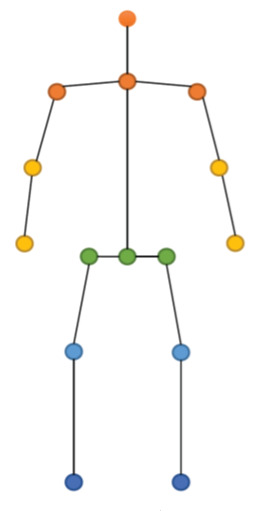
\includegraphics[width=0.3\textwidth]{pose_representation_skeleton}%
	}
	\subcaptionbox{Contour \label{fig:pose_representation_contour}}{%
		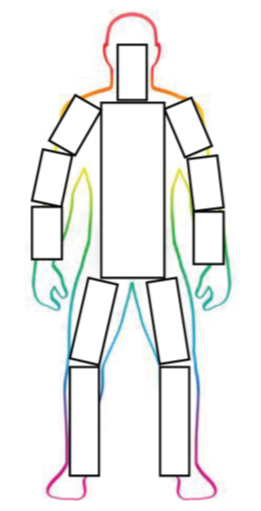
\includegraphics[width=0.3\textwidth]{pose_representation_contour}%
	}
	\subcaptionbox{Volume \label{fig:pose_representation_volume}}{%
		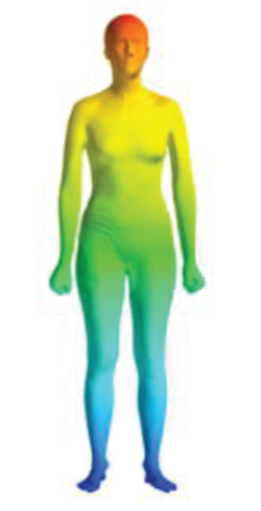
\includegraphics[width=0.3\textwidth]{pose_representation_volume}%
	}
	\caption{Models for pose representation \cite{Zheng2012}}
	\label{fig:pose_representation}
\end{figure}

\begin{figure}
	\centering
	\subcaptionbox{Regression Methods \label{fig:single_pose_estimation_regression_methods}}{%
		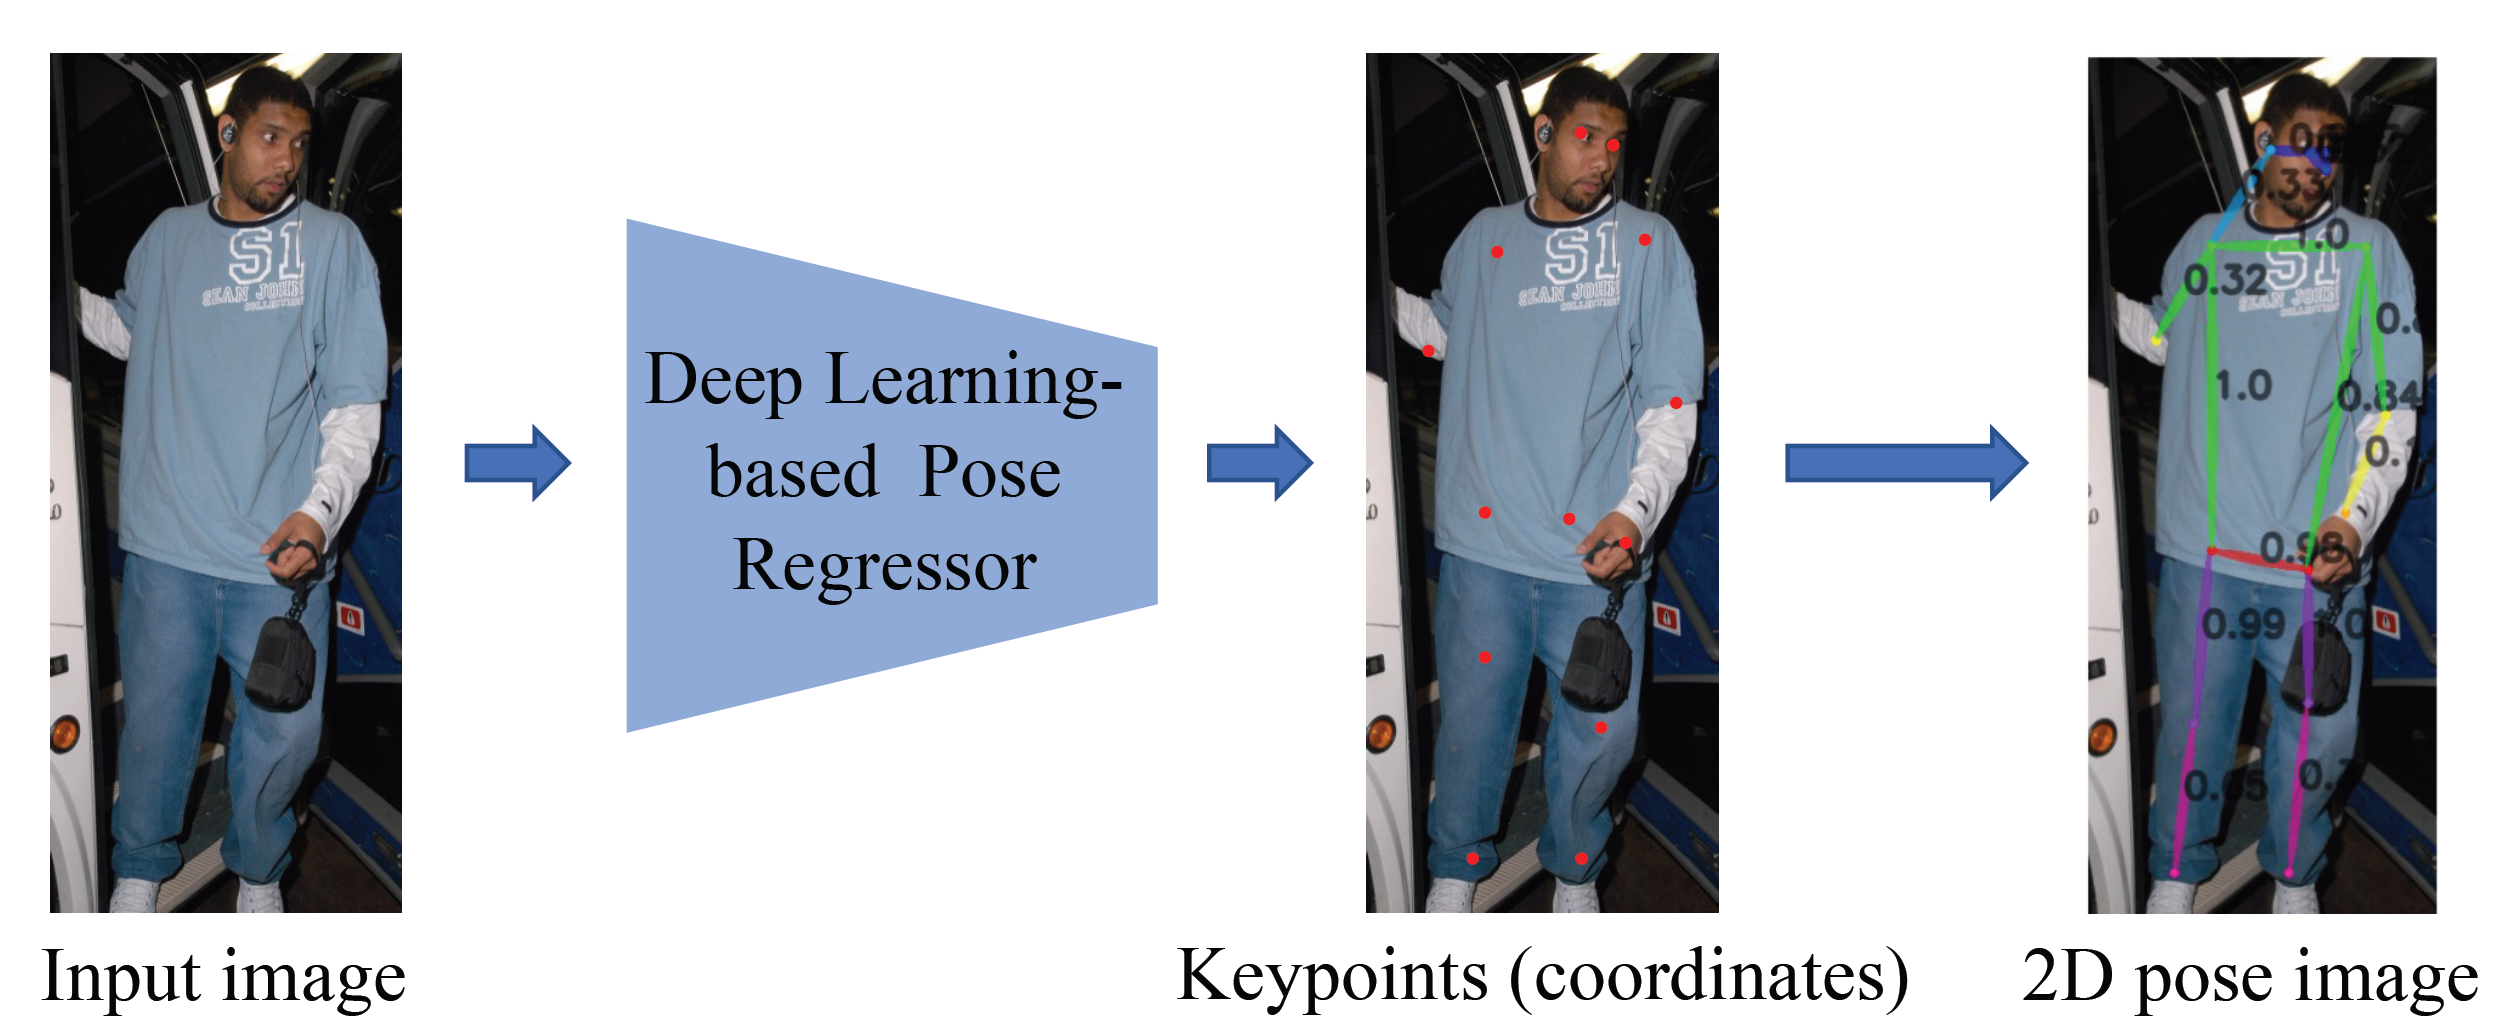
\includegraphics[width=\textwidth]{single_pose_estimation_regression_methods}%
	}
	\subcaptionbox{Heatmap-based Methods \label{fig:single_pose_estimation_heatmap-based_methods}}{%
		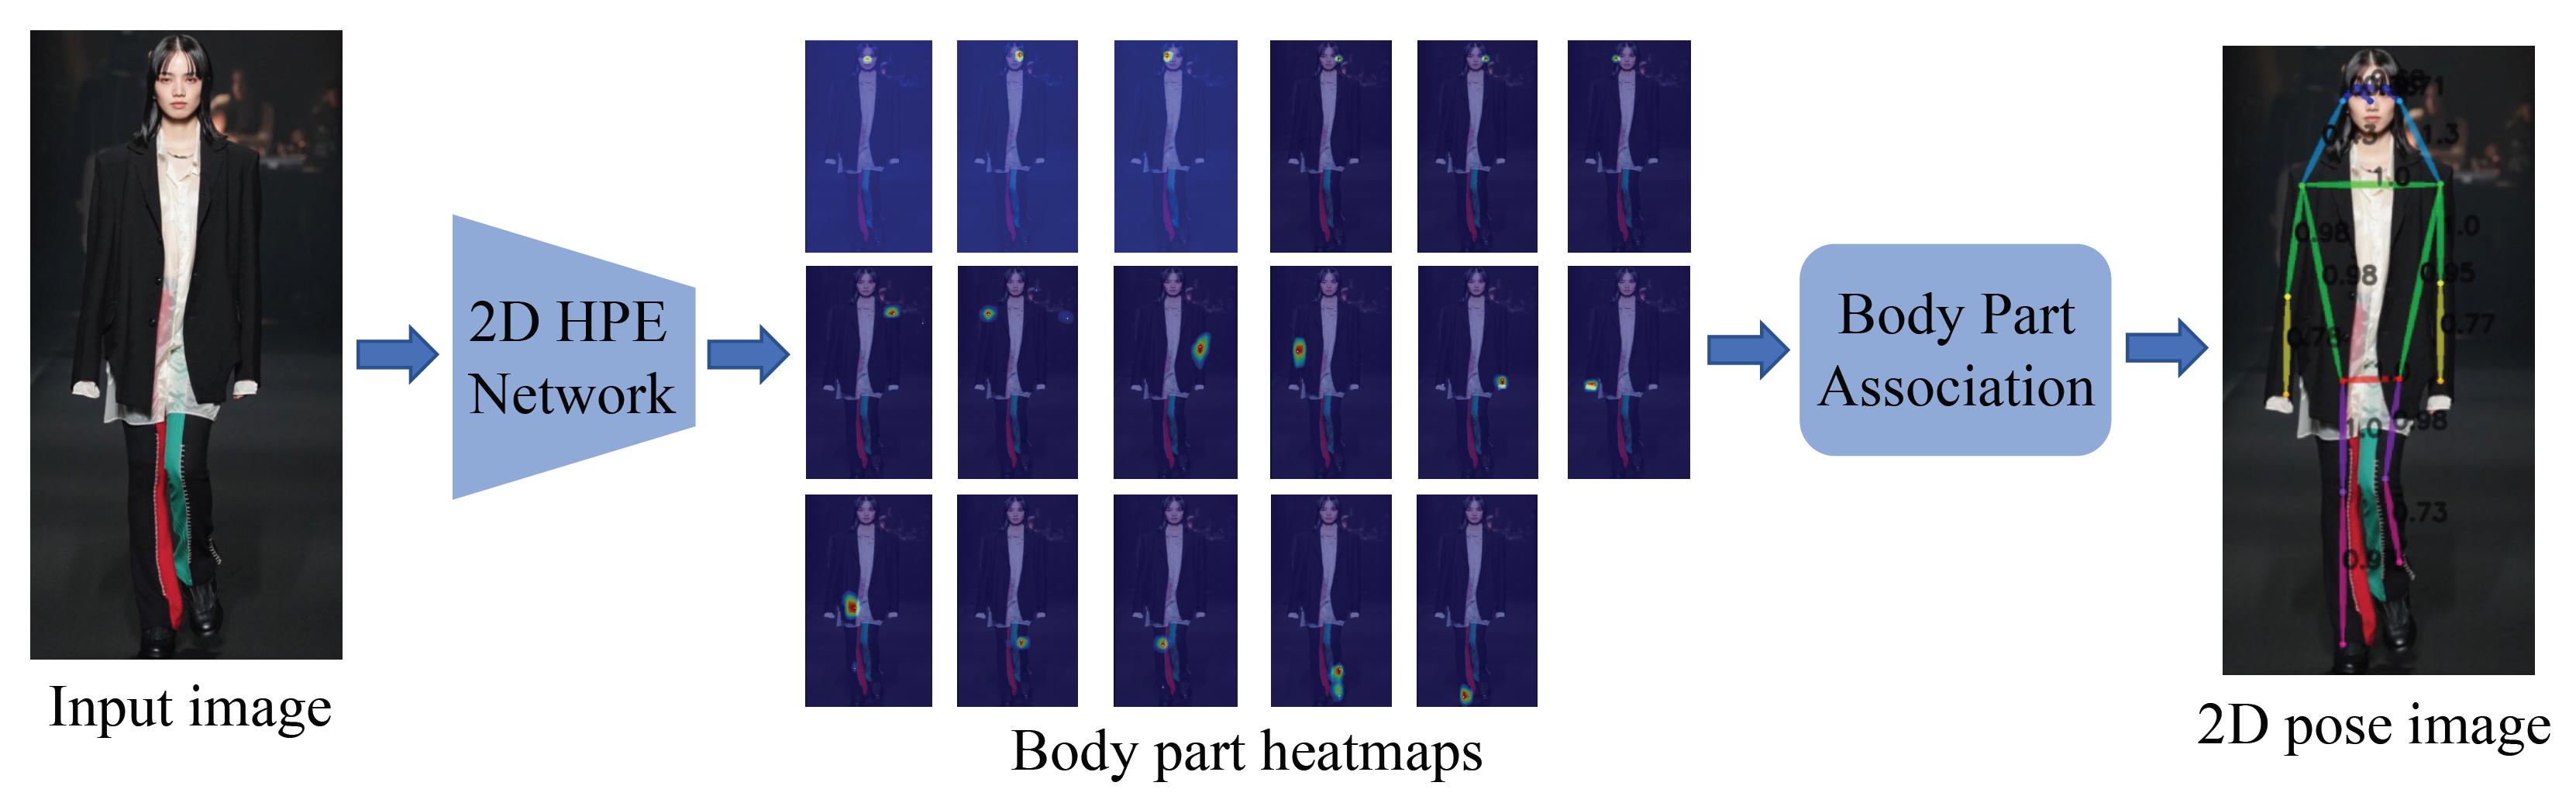
\includegraphics[width=\textwidth]{single_pose_estimation_heatmap-based_methods}%
	}
	\caption{The different methods of single-person human pose estimation.\cite{Zheng2012}}
	\label{fig:single_pose_estimation}
\end{figure}

\begin{figure}
	\centering
	\subcaptionbox{Initial stage \label{fig:single_pose_estimation_deep_pose_initial_stage}}{%
		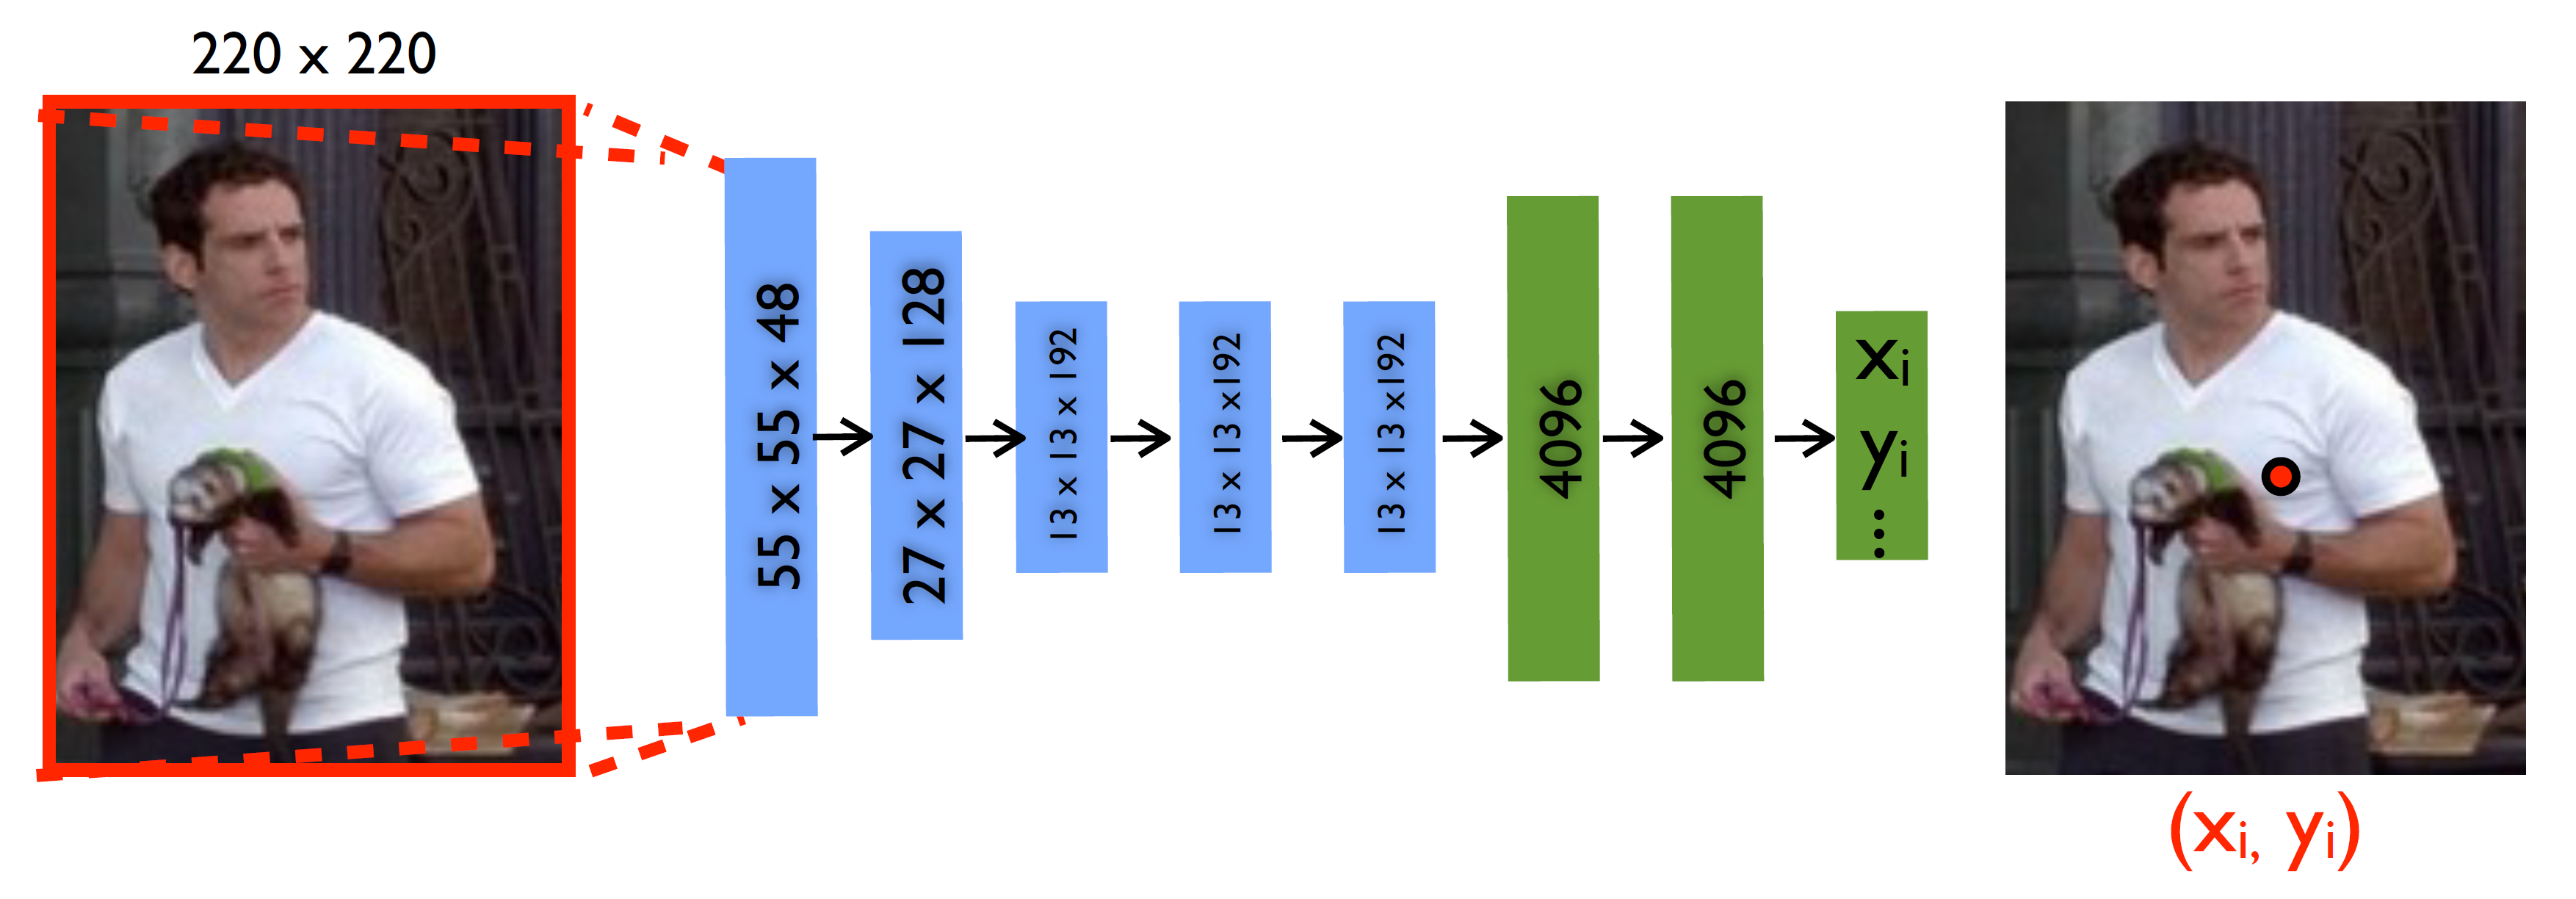
\includegraphics[width=\textwidth]{single_pose_estimation_deep_pose_initial_stage}%
	}
	\subcaptionbox{Stage s \label{fig:single_pose_estimation_deep_pose_stage_s}}{%
		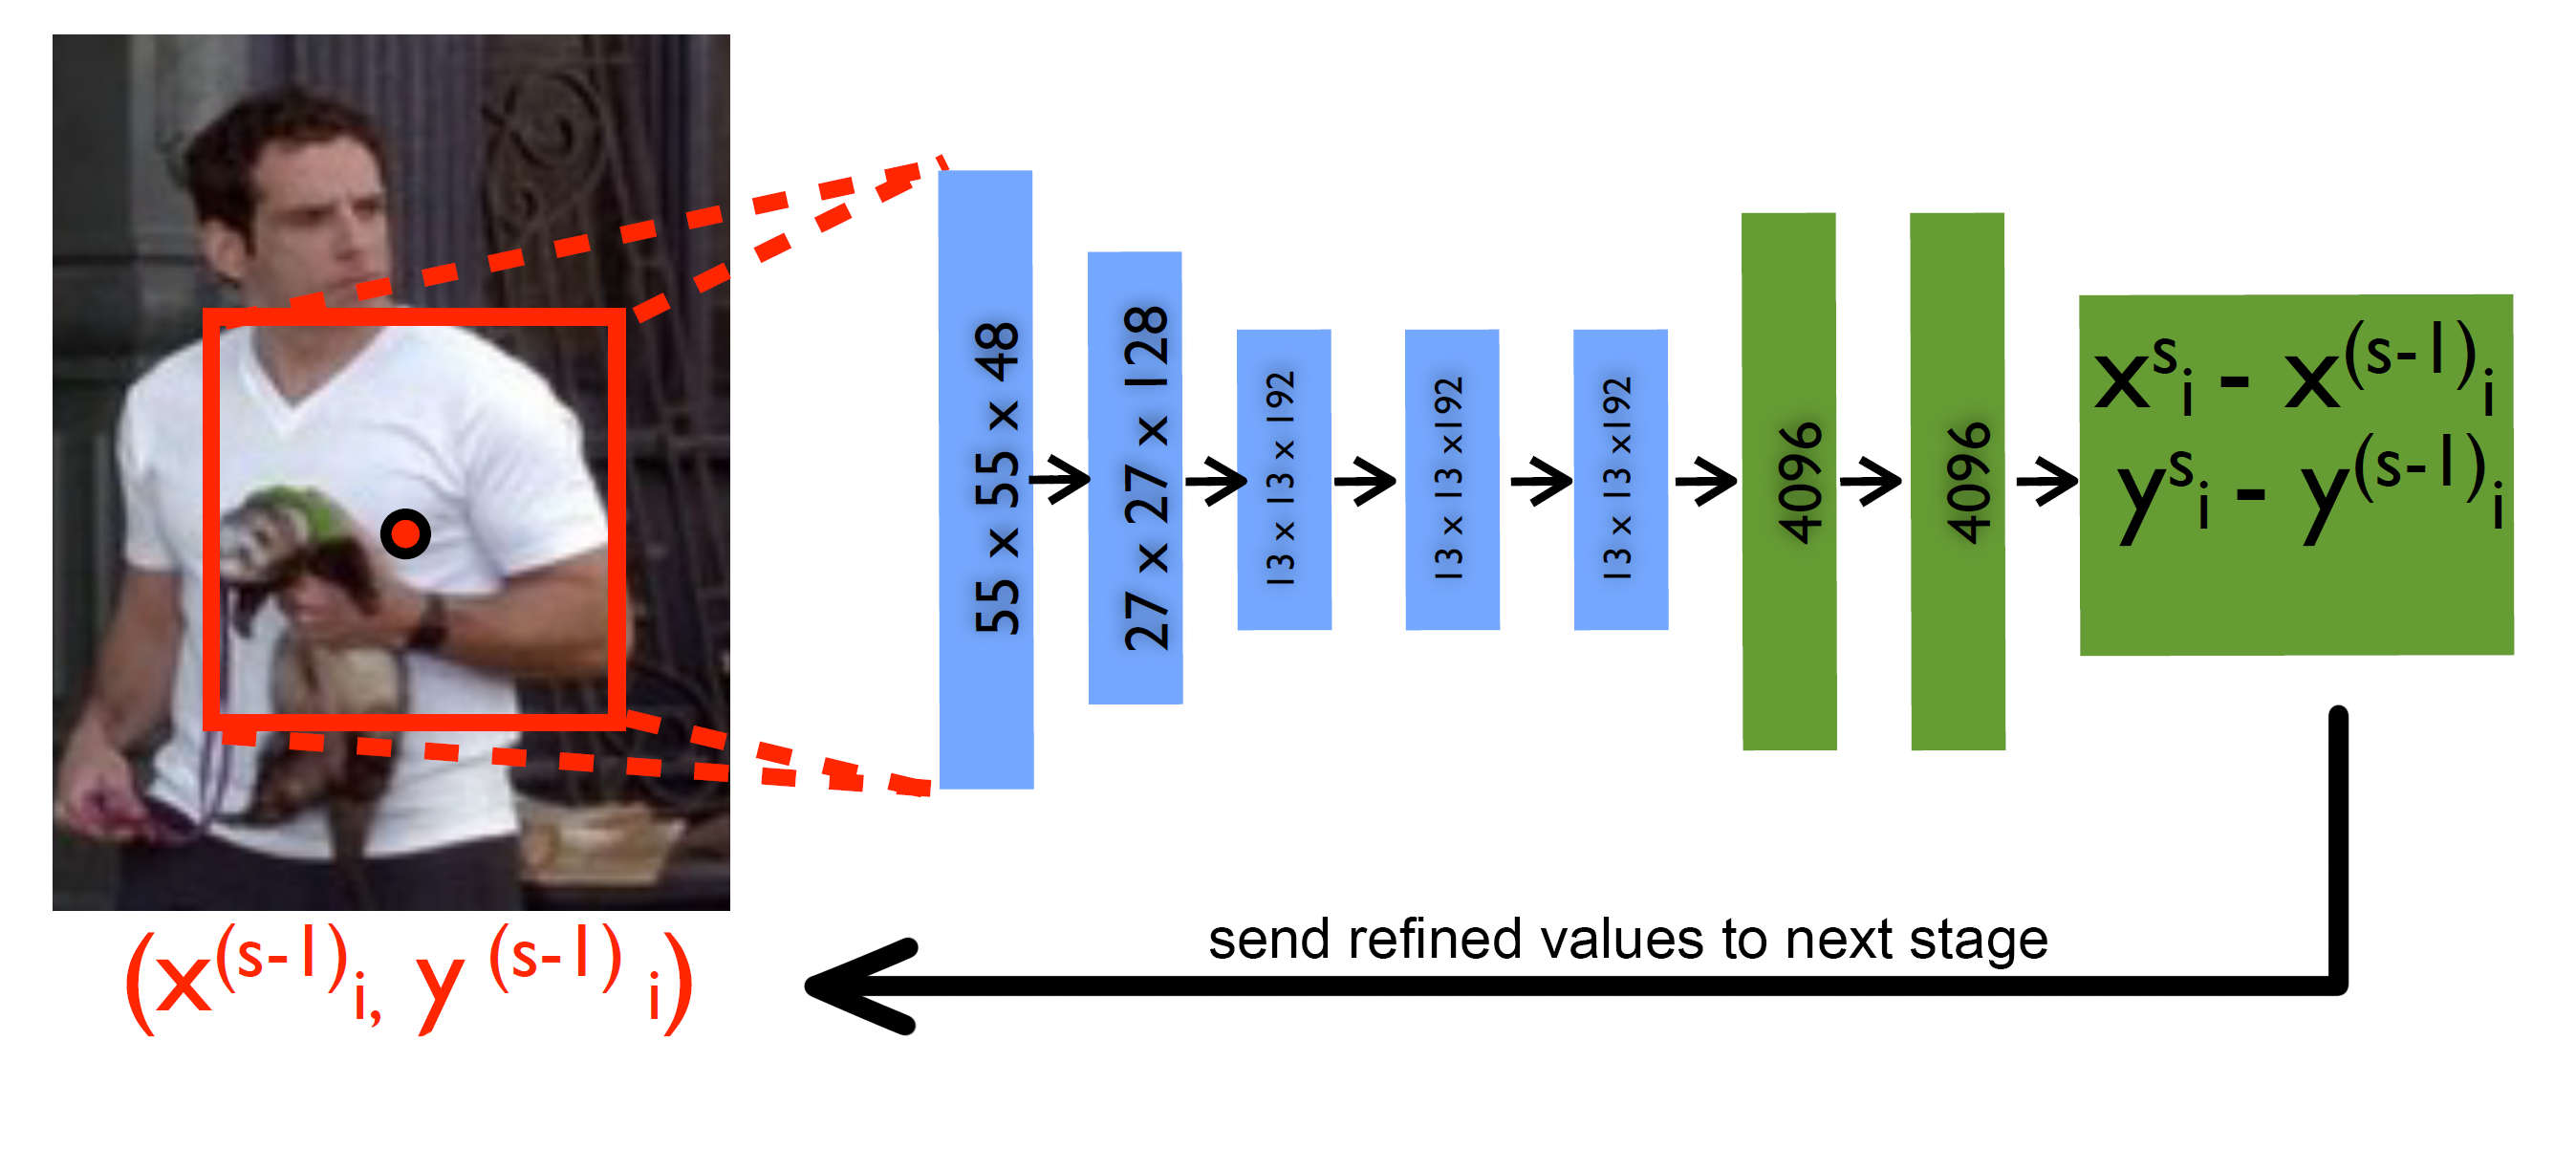
\includegraphics[width=\textwidth]{single_pose_estimation_deep_pose_stage_s}%
	}
	\caption{
		Convolution layers in blue and fully connected layers in green.
		The initial stage is applied to the whole images, while in stage s it will work on a sub-image based on the result of the previous stage.\cite{Toshev2014}
	}
	\label{fig:deep_pose}
\end{figure}

\begin{figure}
	\centering
	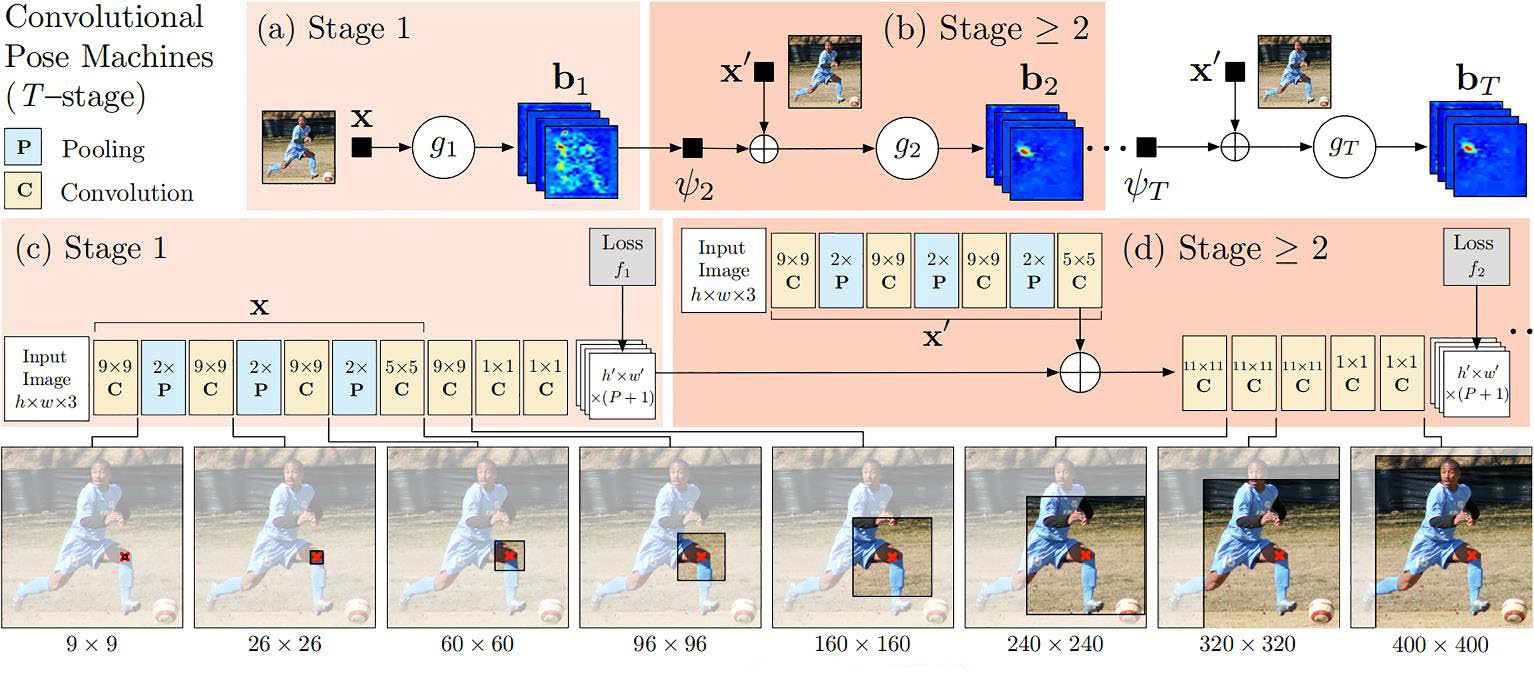
\includegraphics[width=\textwidth]{single_pose_estimation_convolutional_pose_machines}%
	\caption{
		Architecture and receptive fields of \gls{CPMs}. (a) and (b) represent the pose machine architecture.\cite{Ramakrishna2014}
		(c) and (d) show the corresponding convolutional networks used by \gls{CPMs}.\cite{Wei2016}
	}
	\label{fig:convolutional_pose_machines}
\end{figure}

\begin{figure}
	\centering
	\subcaptionbox{Stacked Hourglass \label{fig:single_pose_estimation_stacked_hourglass}}{%
		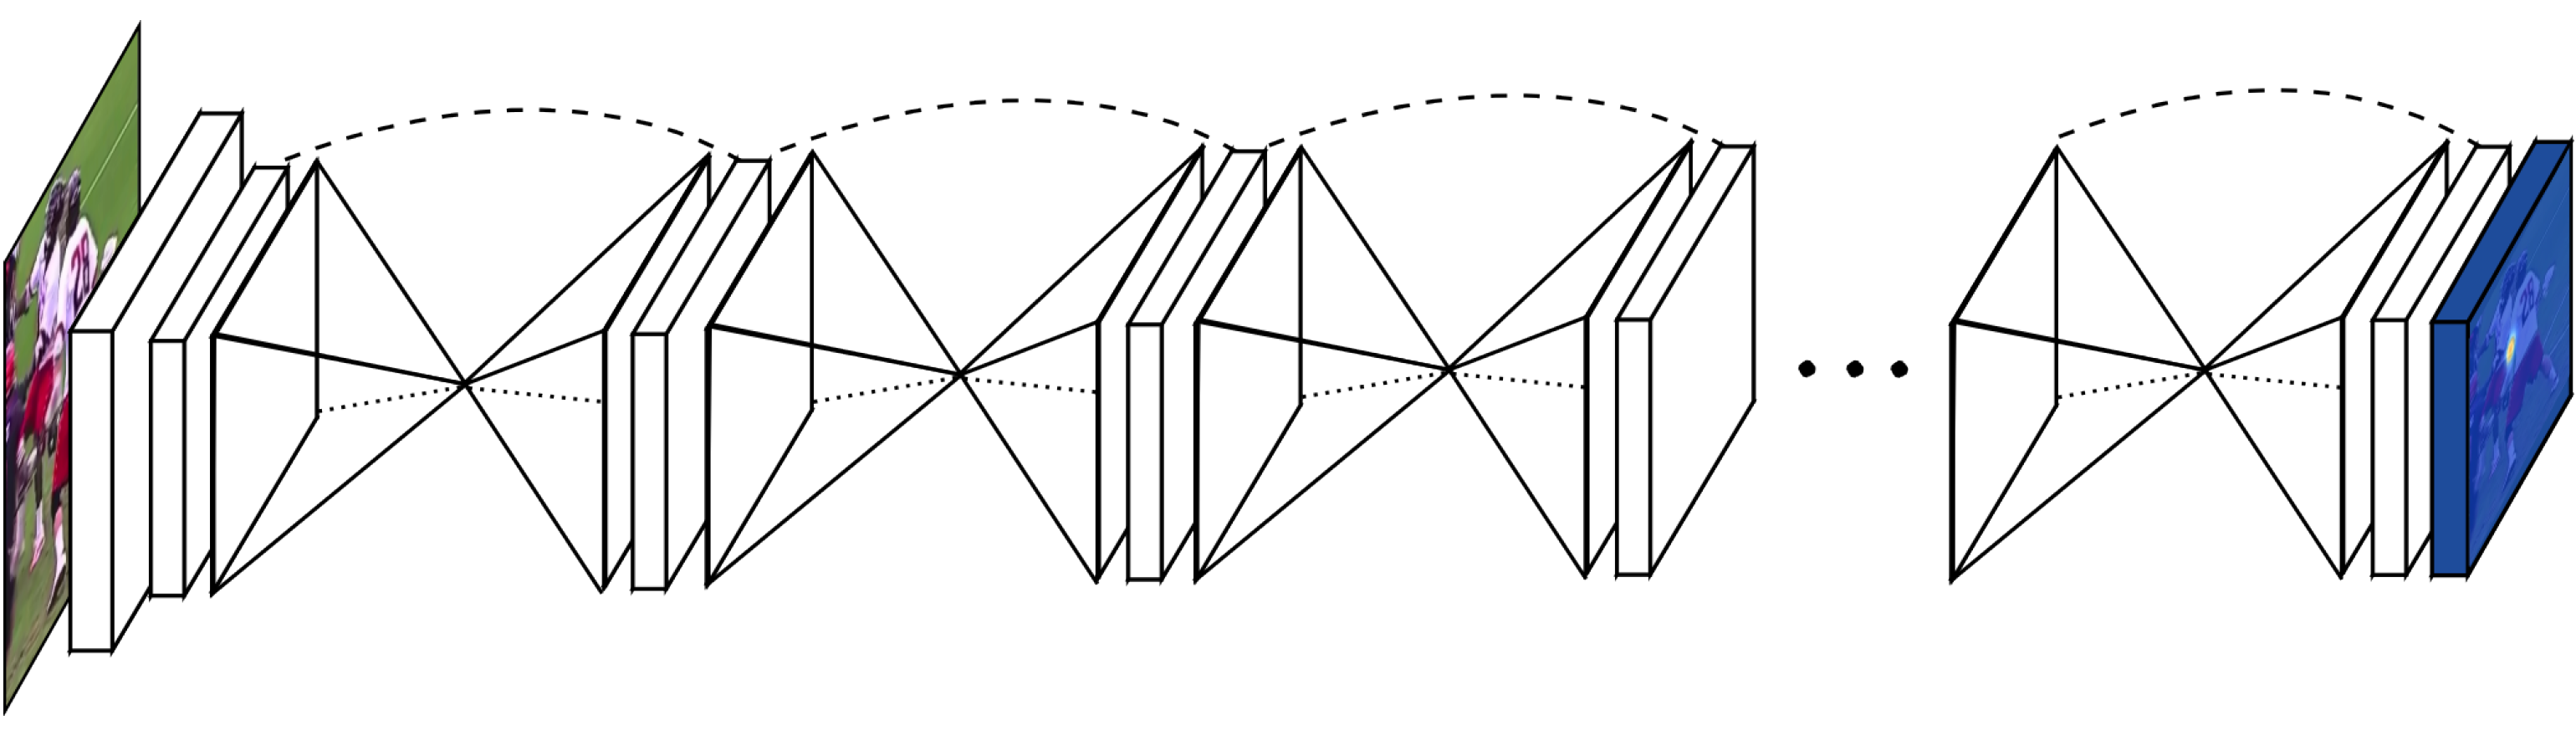
\includegraphics[width=\textwidth]{single_pose_estimation_stacked_hourglass}%
	}
	\subcaptionbox{Hourglass Module \label{fig:single_pose_estimation_hourglass_module}}{%
		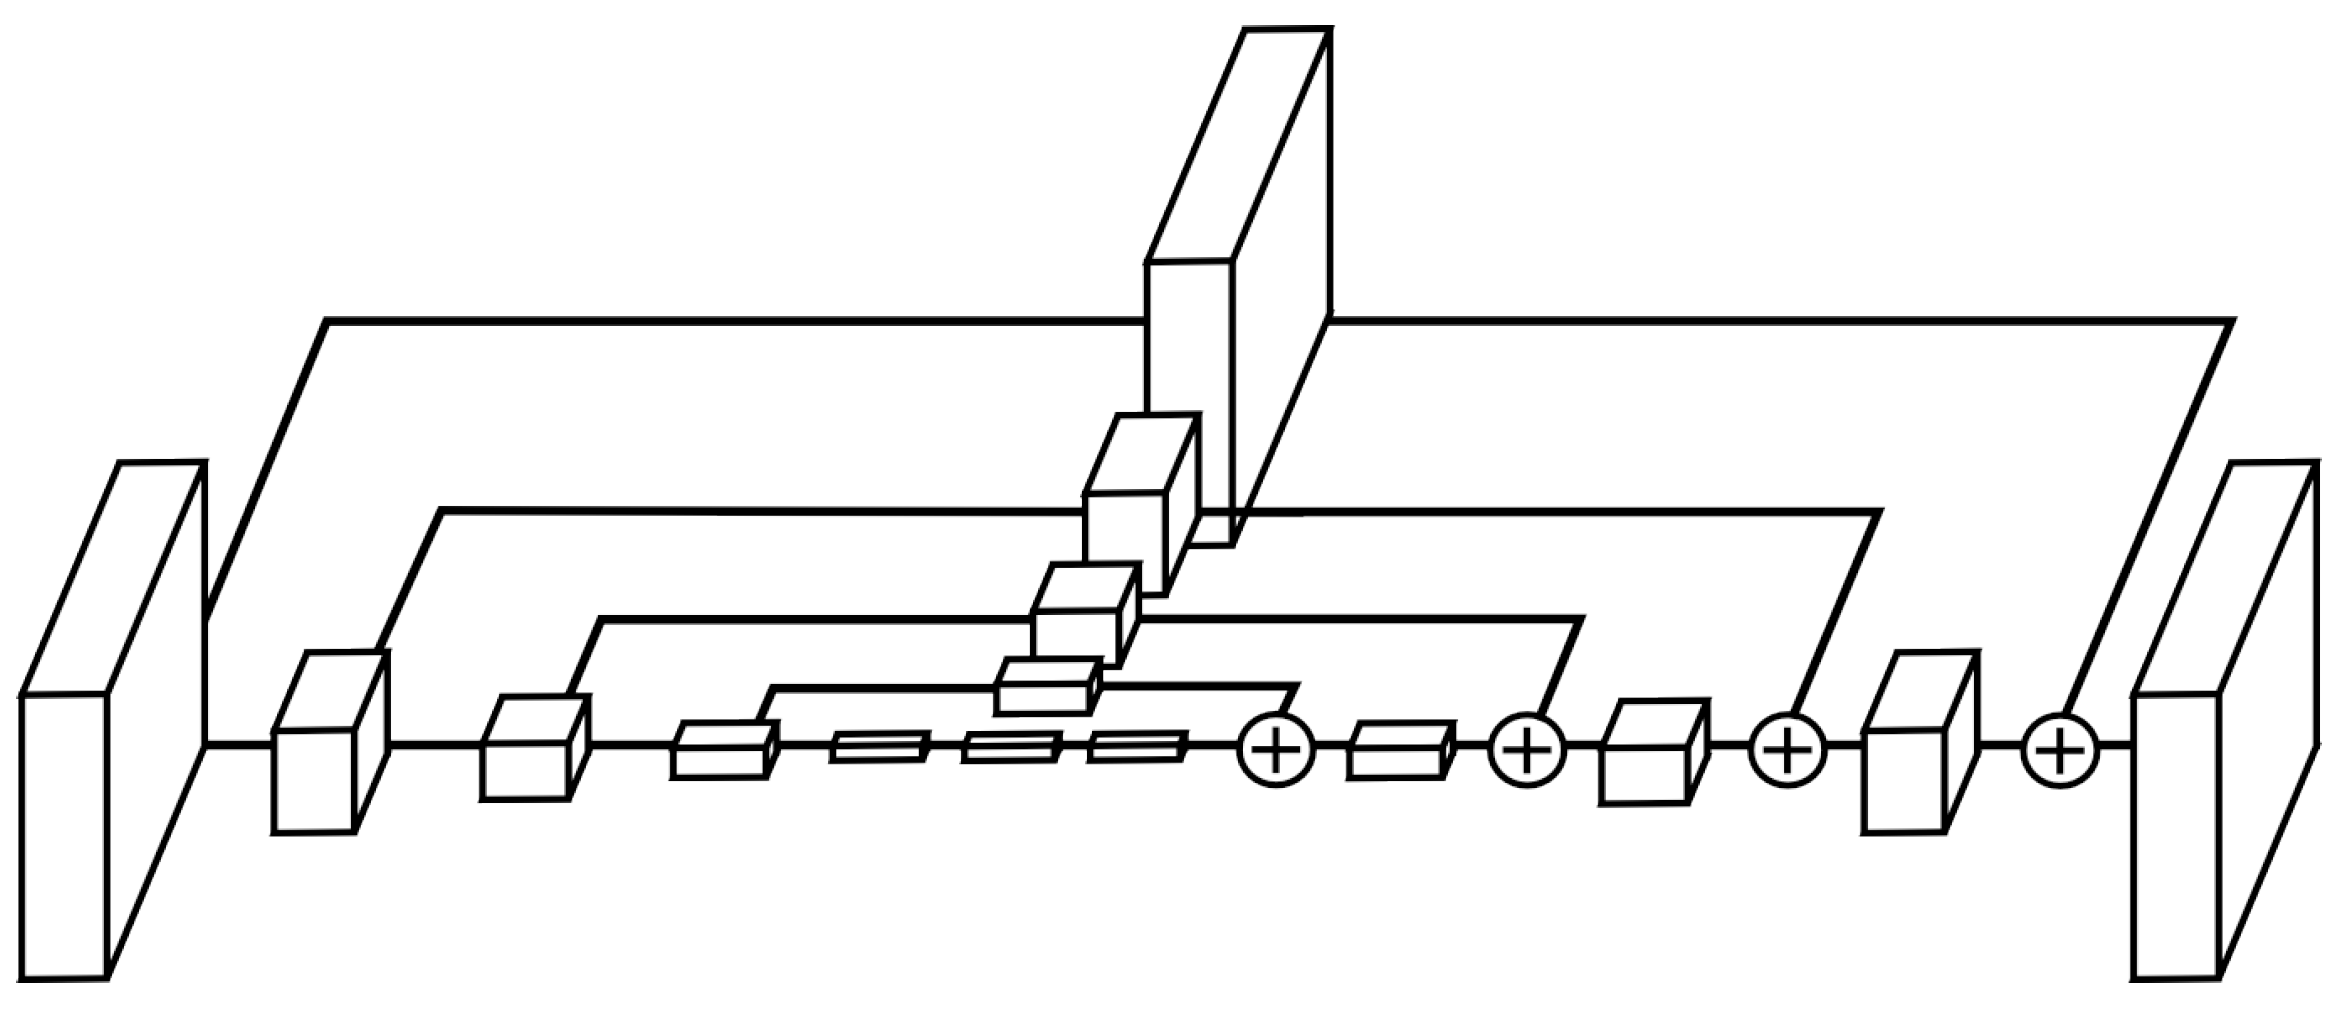
\includegraphics[width=\textwidth]{single_pose_estimation_hourglass_module}%
	}
	\caption{
		The structure of a "stacked hourglass" network and a single "hourglass" module.\cite{Newell2016}
	}
	\label{fig:stacked_hourglass}
\end{figure}

\begin{figure}
	\centering
	\subcaptionbox{HRNet \label{fig:single_pose_estimation_HRNet}}{%
		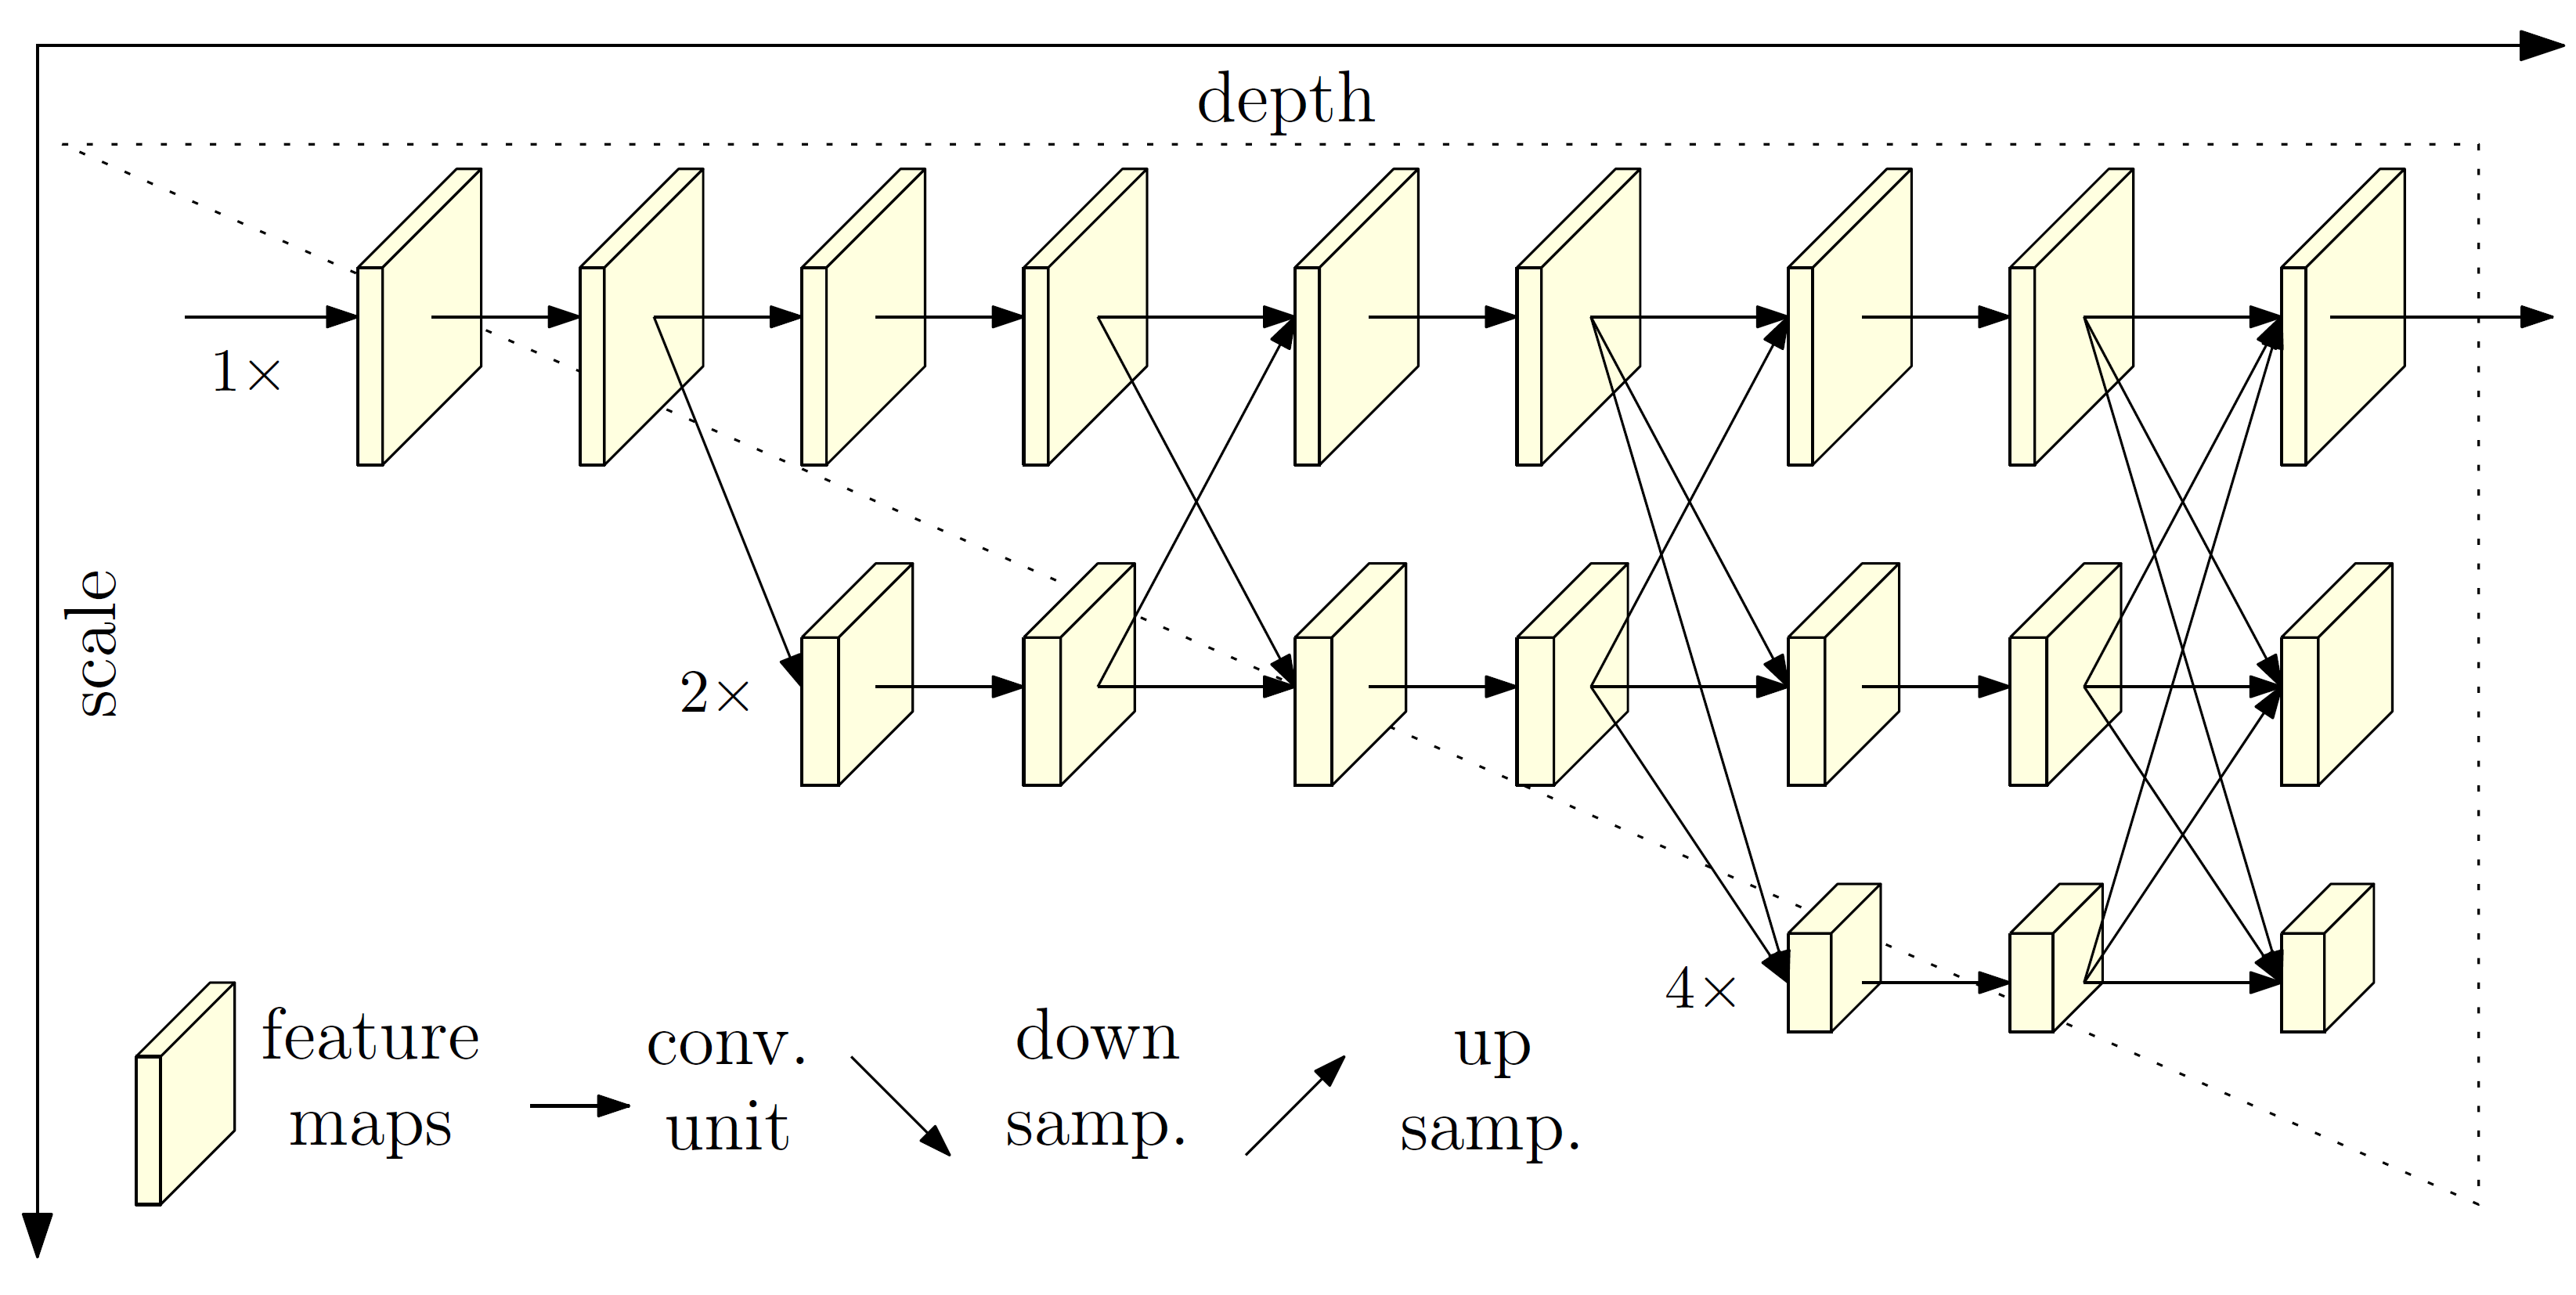
\includegraphics[width=\textwidth]{single_pose_estimation_HRNet}%
	}
	\subcaptionbox{Multi-Scale Fusion \label{fig:single_pose_estimation_multi-scale_fusion}}{%
		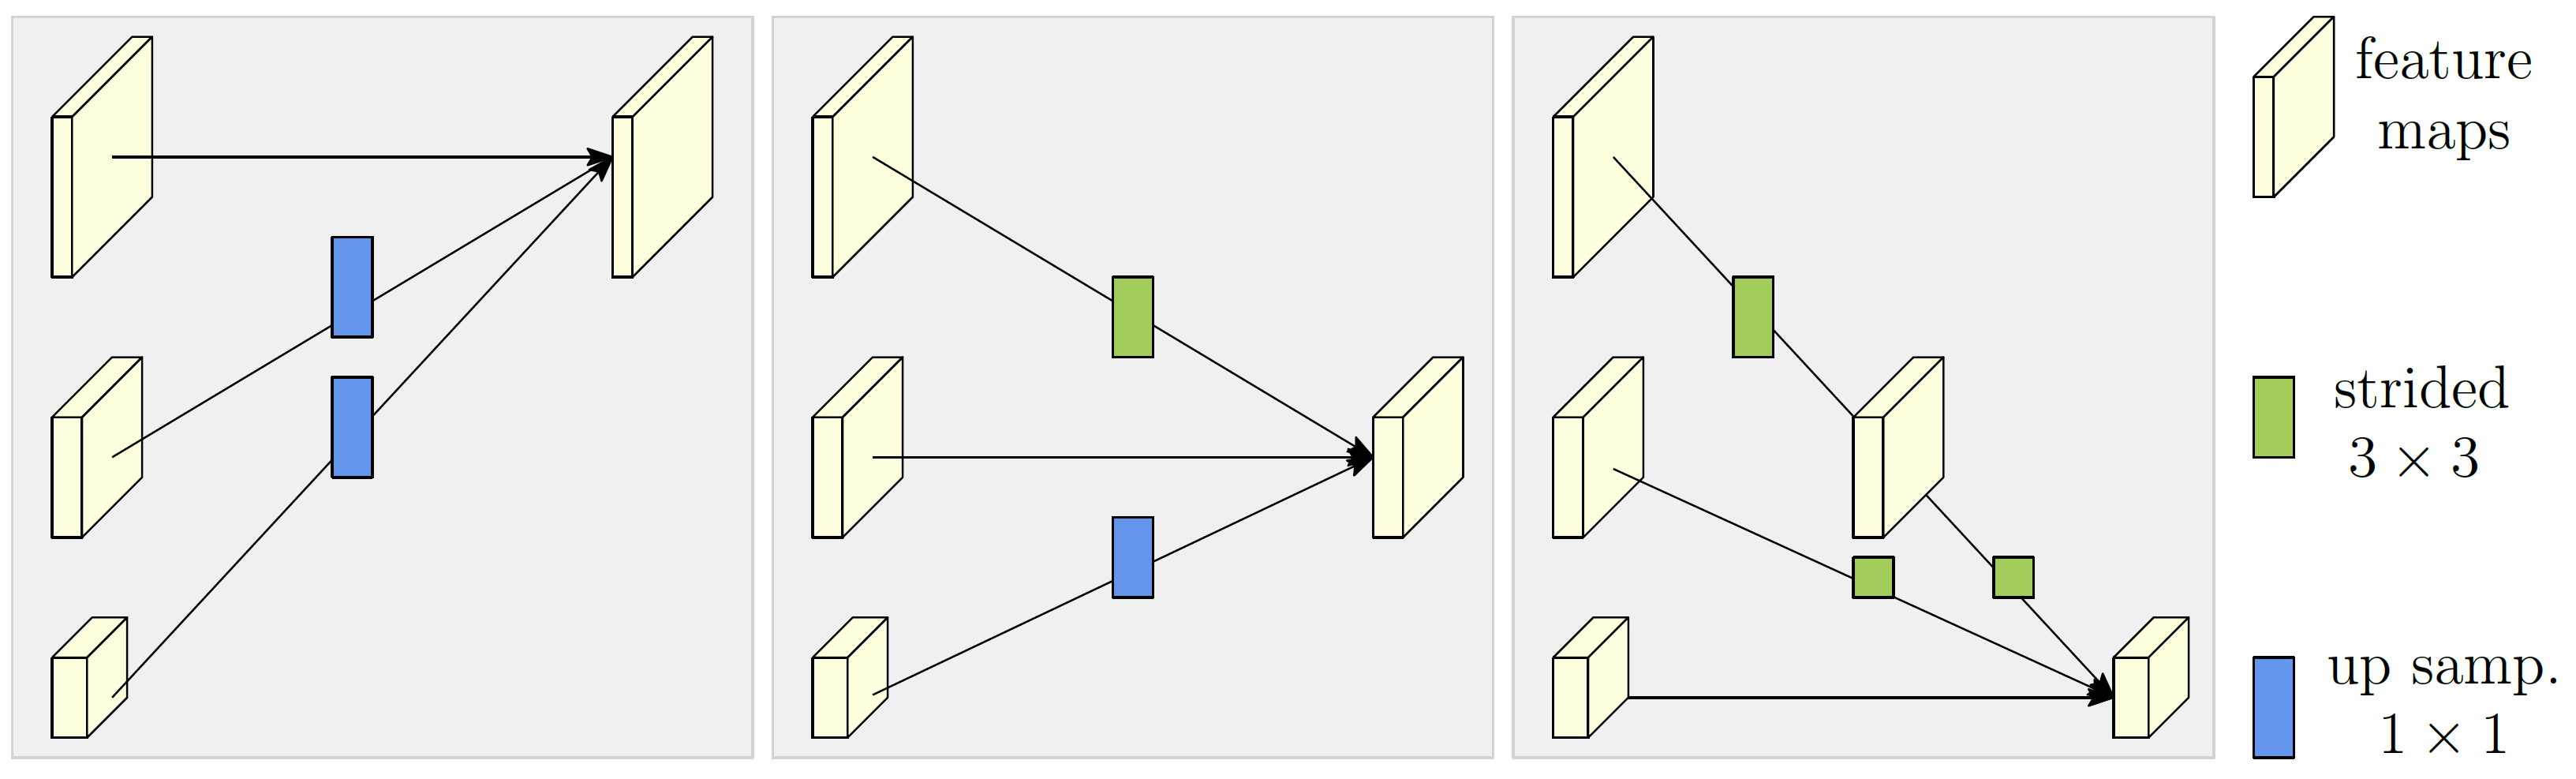
\includegraphics[width=\textwidth]{single_pose_estimation_multi-scale_fusion}%
	}
	\caption{
		The architecture of the High-Resolution network and how it applies multi-scale fusion.\cite{Sun2019}
	}
	\label{fig:HRNet}
\end{figure}

\begin{figure}
	\centering
	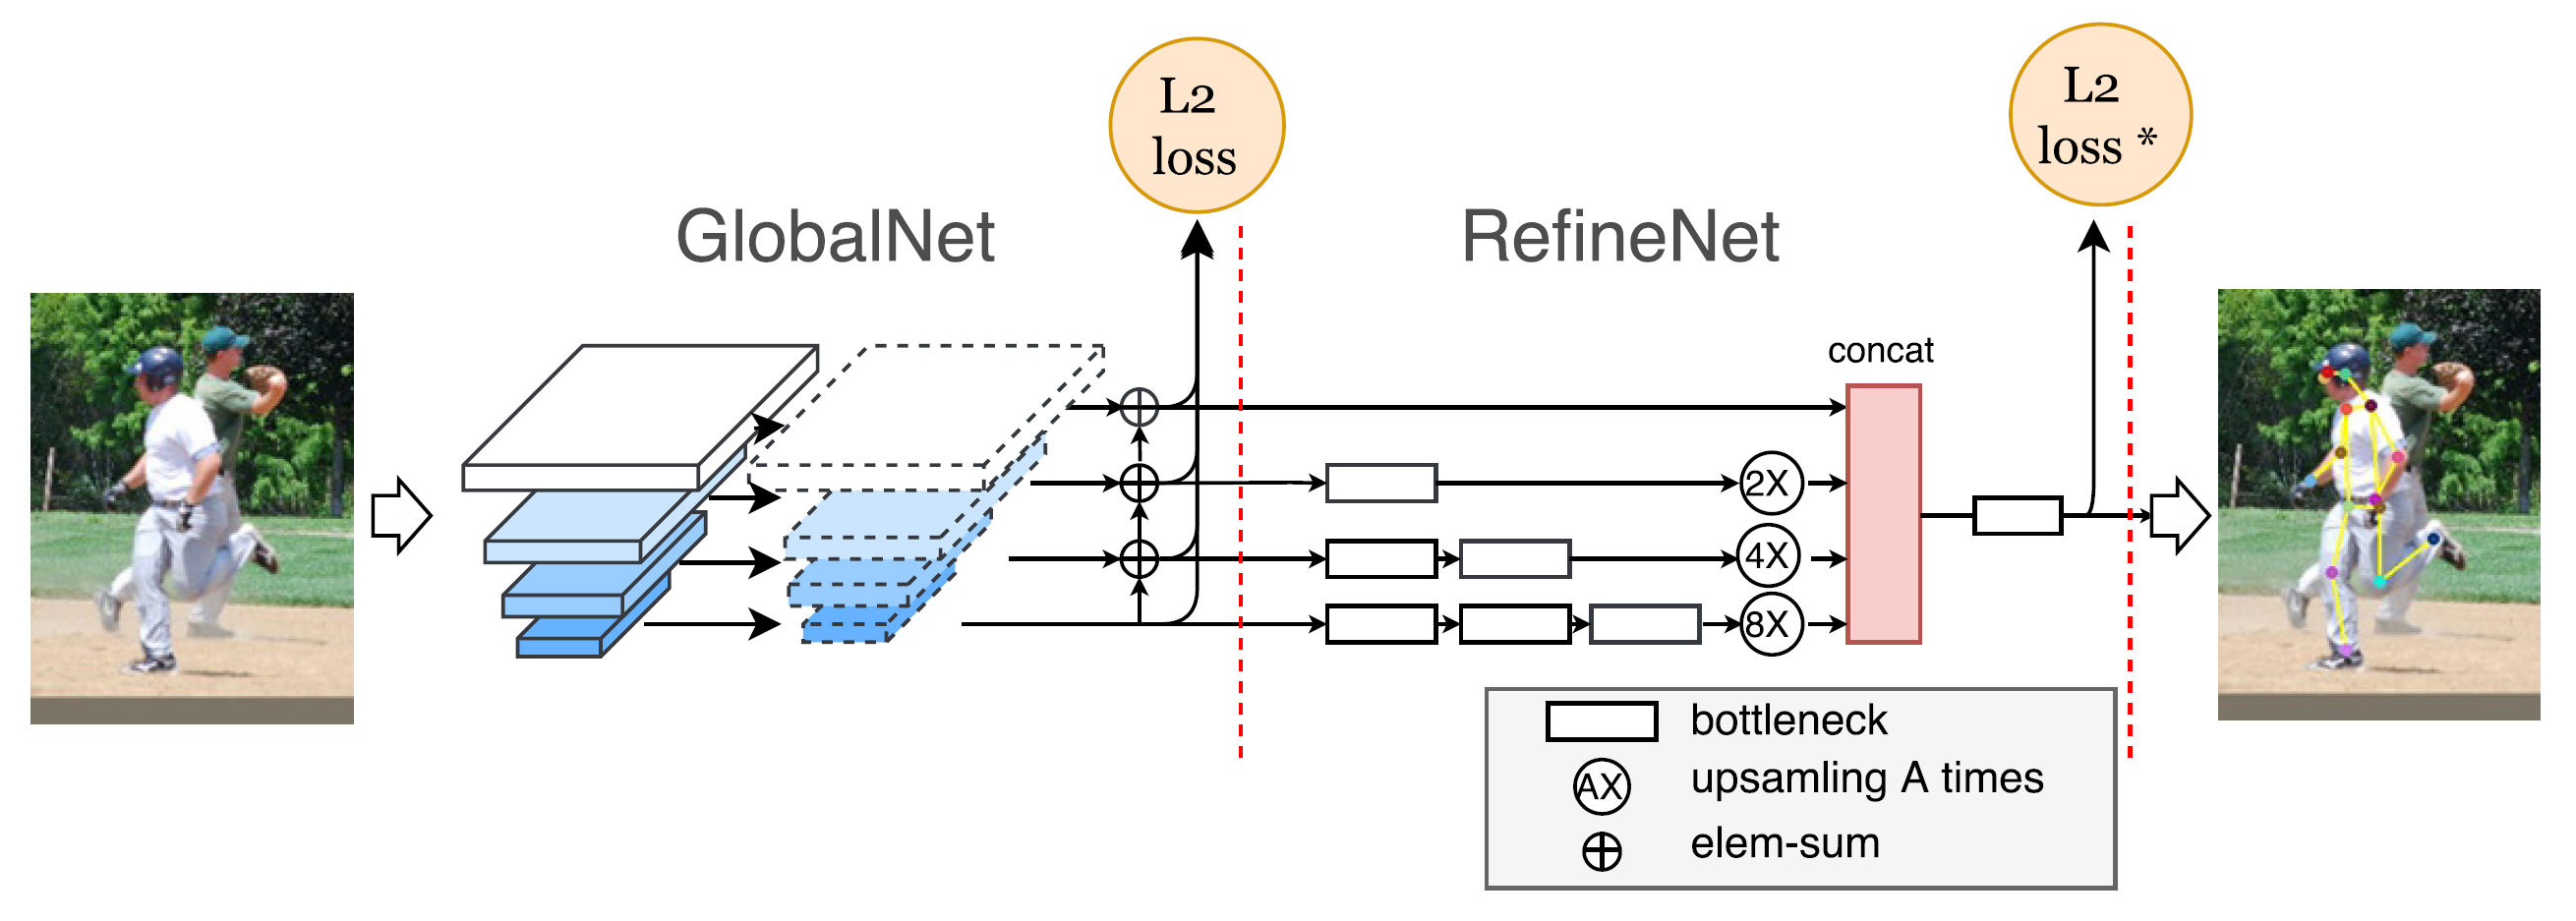
\includegraphics[width=\textwidth]{multi_pose_estimation_cascade_pyramid_network}%
	\caption{
		Cascaded Pyramid Network. “L2 loss*” means L2 loss with online hard keypoints mining.\cite{Chen2017}
	}
	\label{fig:cascade_pyramid_network}
\end{figure}

\section{Image Style Transfer}
Image Style Transfer is the technique of applying the style of one image to the content of another.
Classically this was a problem reserved for only artists, but more recently this has also interested computer scientists.
There are several different ideas on how this can be achieved,
ranging from how to separate the style from the content, to how well an algorithm can generalize.
An overview of all the different challenges and solutions will be given in this chapter.

\subsection{Datasets}
Due to a lack of benchmark datasets, multiple papers will mix and match from different datasets, like \gls{COCO} or ImageNet \cite{Deng2009}.

\textbf{Cityscape Dataset \cite{Cordts2016}} consists of 2975 images of cityscapes with semantic annotations.

\textbf{Facades Dataset \cite{Tylecek2013}} consists of 400 images of building facades with architectural annotations.

\textbf{Maps Dataset \cite{Isola2016}} consists of 1096 images of maps and areal photos gathered from Google Maps around New York City.

\textbf{Edges2shoes Dataset \cite{Yu2014}} consists of 50,000 paired images between edges and photos of shoes.

\textbf{Edges2handbags Dataset \cite{Zhu2016}} consists of 137,000 paired images between edges and photos of handbags.

\textbf{Season transfer Dataset \cite{Zhu2017}} consists of 2127 images of Yosemite during summer and winter downloaded from Flickr.

\textbf{Night2Day Dataset \cite{Laffont2014}} consists of 20,000 images taken from time-lapse datasets and annotated through crowdsourcing.

\textbf{WikiArt Dataset \cite{Tan2018}} consists of 80,000 fine-art paintings.
All are annotated for 27 styles, 60,000 are annotated for 20 genres and 20,000 for 23 artists.


\subsection{Optimization-based Networks}
Gatys et al. \cite{Gatys2016} introduce deep neural networks to image style transfer.
Using a modified VGG-network \cite{Simonyan2015}, they extract the features of an image by reconstructing the content from the feature maps in the higher layers on a white noise image.
The same is done for the style of the other image.
It extracts the style representation of the image by using the Gram matrix to represent style features of the image and then reconstructs it on the same white noise image.
The Gram matrix is the vector product of two sets of vectorized feature maps.
This method is shown in \ref{fig:style_transfer_algorithm}.
They remark that the resolution of the images affects the performance of the algorithm and is thus restricted to low resolutions.
At the same time, the synthesized images contain some low-level noise, but this can possibly be removed with a denoiser.

\subsection{Feed-forward Generation Networks}
To improve the performance, Ulyanov et al. \cite{Ulyanov2016} suggest the use of a feed-forward generation network instead of backpropagation
Backpropagation requires an iterative process to change the pixel values to match the desired statistics.
A feed-forward network can do this in a single evaluation.
To train such a network they use a pre-trained network for image classification, and calculate a texture and content loss like \cite{Gatys2016}, as shown in \ref{fig:style_transfer_generator_network_ulyanov}.
Johnson et al. \cite{Johnson2016} propose a very similar method as can be seen in \ref{fig:style_transfer_generator_network_johnson}

Since their contribution did increase the speed, but at the expense of quality, Ulyanov et al. \cite{Ulyanov2017} suggest further improvements to their network.
First, they replace \gls{BN} \cite{Ioffe2015} with \gls{IN} which alone has a significant impact on quality as can be seen in \ref{fig:style_transfer_ulyanov_BN_IN_comparison}.
Second, they learn the generator to sample from the Julesz ensemble \cite{Zhu2000} which improves variation in the outputs.

Dumoulin et al. \cite{Dumoulin2016} note that previous feed-forward networks are limited to one style.
In order to facilitate many different styles, there would need to be a network trained separately for each which limits the applications for mobile devices.
In order to make the network more memory efficient, they propose a conditional style transfer network; given a content image and a style name, it transforms the image to the corresponding style.
They argue that after normalization each style can be distinguished by specializing scaling and shifting parameters.
They call this \gls{CIN}.
Since it only changes the scale and shift parameters for different styles, the network requires fewer parameters.
Of the 1.6M parameters, only 3K are needed for the different styles.

Another network that puts a focus on multiple styles comes from Chen et al. \cite{Chen2017}.
They propose a StyleBank, which can store multiple convolution filter banks each representing a different style.
They use an auto-encoder network with in between a StyleBank layer.
During training, for each $T+1$ iterations the entire network is first trained with a perception loss for the first $T$ iterations.
Then only the auto-encoder network is trained with a \gls{MSE} loss.
This way the auto-encoder only retains the content and the StyleBank layer only the different styles.
This also allows to lock the encoder and decoder to learn a new style afterwards.

While \gls{CIN} allows for multiple styles, it's still limited to the ones that were seen during training.
Huang et al. \cite{Huang2017} try to remedy this by introducing an \gls{AdaIN} layer.
Unlike the other normalization techniques, \gls{AdaIN} does not have affine parameters, and will adaptively compute these from the style image.
\ref{fig:style_transfer_unseen_style} shows how well the different networks can handle unseen styles.

\subsection{Generative Adversarial Networks}
With the introduction of \glspl{GAN}, the quality of generative models have greatly increased.
It is not surprising then that this got picked up in research for \gls{NST}.

Among the first was Isola et al. \cite{Isola2016} who use a \gls{cGAN}.
With \gls{cGAN}, the generator network has an extra input which here is the image to be translated.
They use the network from \cite{radford2016} which uses modules of the form convolution-BatchNorm-ReLu\cite{Ioffe2015}.
Additionally, in order to pass shared features in the generator they add skip connections like with "U-Net" \cite{Ronneberger2015}.
For the discriminator, which they call PatchGAN, they validate $N\times N$ patches and take the average as output.
They take this loss together with the $L1$ loss because $L2$ loss produces blurry results.

This still requires paired training samples, while Taigman et al. \cite{Taigman2016} are doing research in unsupervised domain transfer.
Domain transfer can be used for \gls{NST}, but this is not possible the other way around.
Their network uses a encoder-decoder as the generator and they assume that $f(x)$ is constant between 2 domains.
The discriminator has a ternary output and distinguishes between real, fake and reconstruction.
They add several new loss functions which check the consistency between the 2 domains (consistency loss) and if $G$ performs perfect reconstruction (reconstruction loss).
This can be seen in \ref{fig:style_transfer_algorithm_taigman}.
For $f$, they use a pre-trained network that is trained on paired samples.

In order to make the network completely unsupervised, Yi et al.\cite{Yi2017} propose DualGAN, Kim et al. \cite{Kim2017} DiscoGAN and Zhu et al. \cite{Zhu2017} CycleGAN, which are all 3 essentially the same proposal.
The entire model consists of 2 cycle-consistent networks where each translates from one domain to the other.
A cycle-consistent network will first translate the input to target domain and then back to the original domain.
Each domain has a discriminator which compares the real input from one network with the fake from the other; the adversarial loss. As seen in \ref{fig:style_transfer_algorithm_discogan}.
In addition to this there's a cycle-consistency loss, which is the \gls{MSE} between the input and the reconstructed image as you can see in \ref{fig:style_transfer_algorithm_cyclegan}.
The goal is to minimize the adversarial and cycle-consistency losses, while maximizing the discriminators' accuracy.
Zhu et al. \cite{Zhu2017} also introduce an identity loss.

Liu et al. \cite{Liu2017} introduce the latent space assumption which assumes that paired images from different domains can be mapped to a shared latent space with the same latent representation.
The network consists of 2 domain image encoders $E\textsubscript{$1$}$ and $E\textsubscript{$2$}$, 2 domain image generators $G\textsubscript{$1$}$ and $G\textsubscript{$2$}$, and 2 domain discriminators $D\textsubscript{$1$}$ and $D\textsubscript{$2$}$.
As can be seen in \ref{fig:style_transfer_algorithm_unit}.
The encoders and generators are paired and form a \gls{VAE} \cite{kingma2022}.
The encoder maps the input to latent space, and the generator reconstructs the image.
This is the reconstruction loss.
They use weight-sharing, which shares the weight of the last 2 layers of the encoders and of the first 2 layers of the generators.
The generators and discriminators are paired to form a \gls{GAN}.
The generator can also construct an image from the latent code from the other encoder's input.
This image is used to train the \gls{GAN}.
They also show that the shared-latent space assumption implies cycle-consistency, which is the final loss function of the network.



\begin{figure}
	\centering
	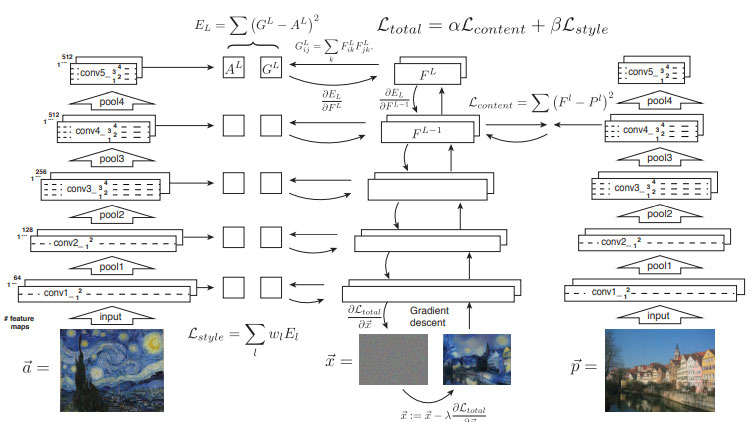
\includegraphics[width=\textwidth]{style_transfer_algorithm}%
	\caption{
		Style transfer algorithm. (Gatys et al. \cite{Gatys2016}).
	}
	\label{fig:style_transfer_algorithm}
\end{figure}
\begin{figure}
	\centering
	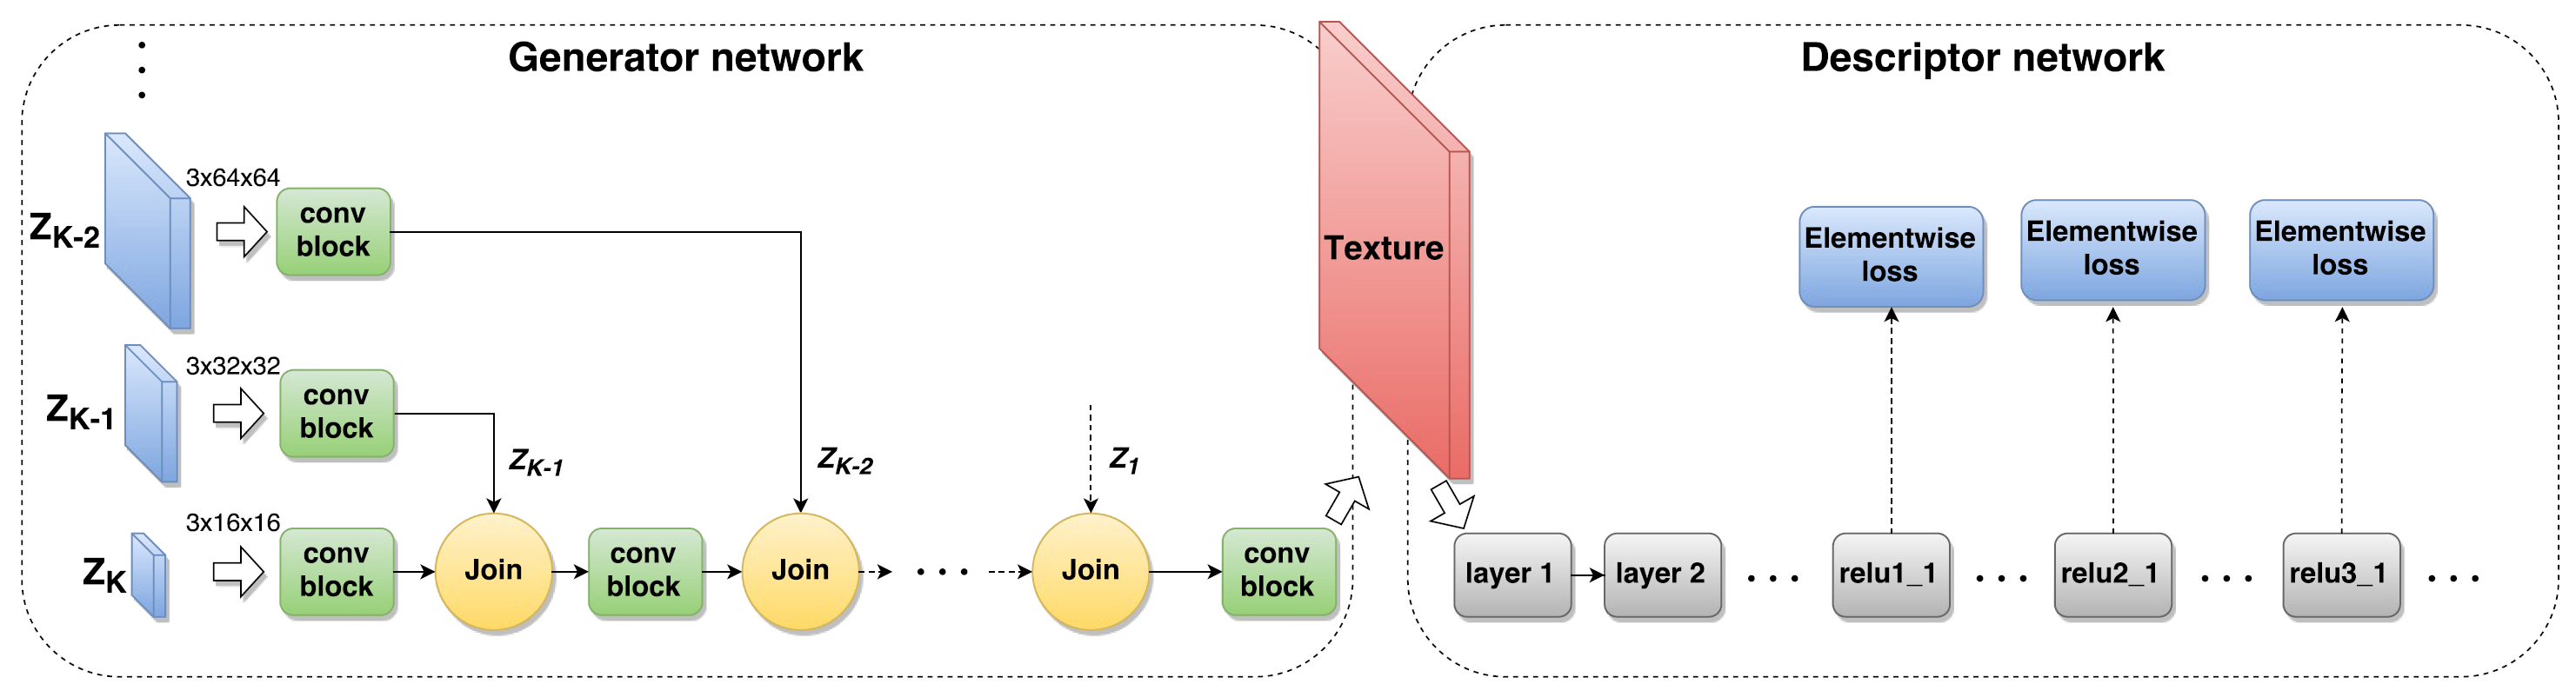
\includegraphics[width=\textwidth]{style_transfer_generator_network_ulyanov}%
	\caption{
		A texture network by Ulyanov et al. \cite{Ulyanov2016}.
		The generator network (left) is the only one that changes.
		The descriptor network (right) is used to calculate the loss.
	}
	\label{fig:style_transfer_generator_network_ulyanov}
\end{figure}
\begin{figure}
	\centering
	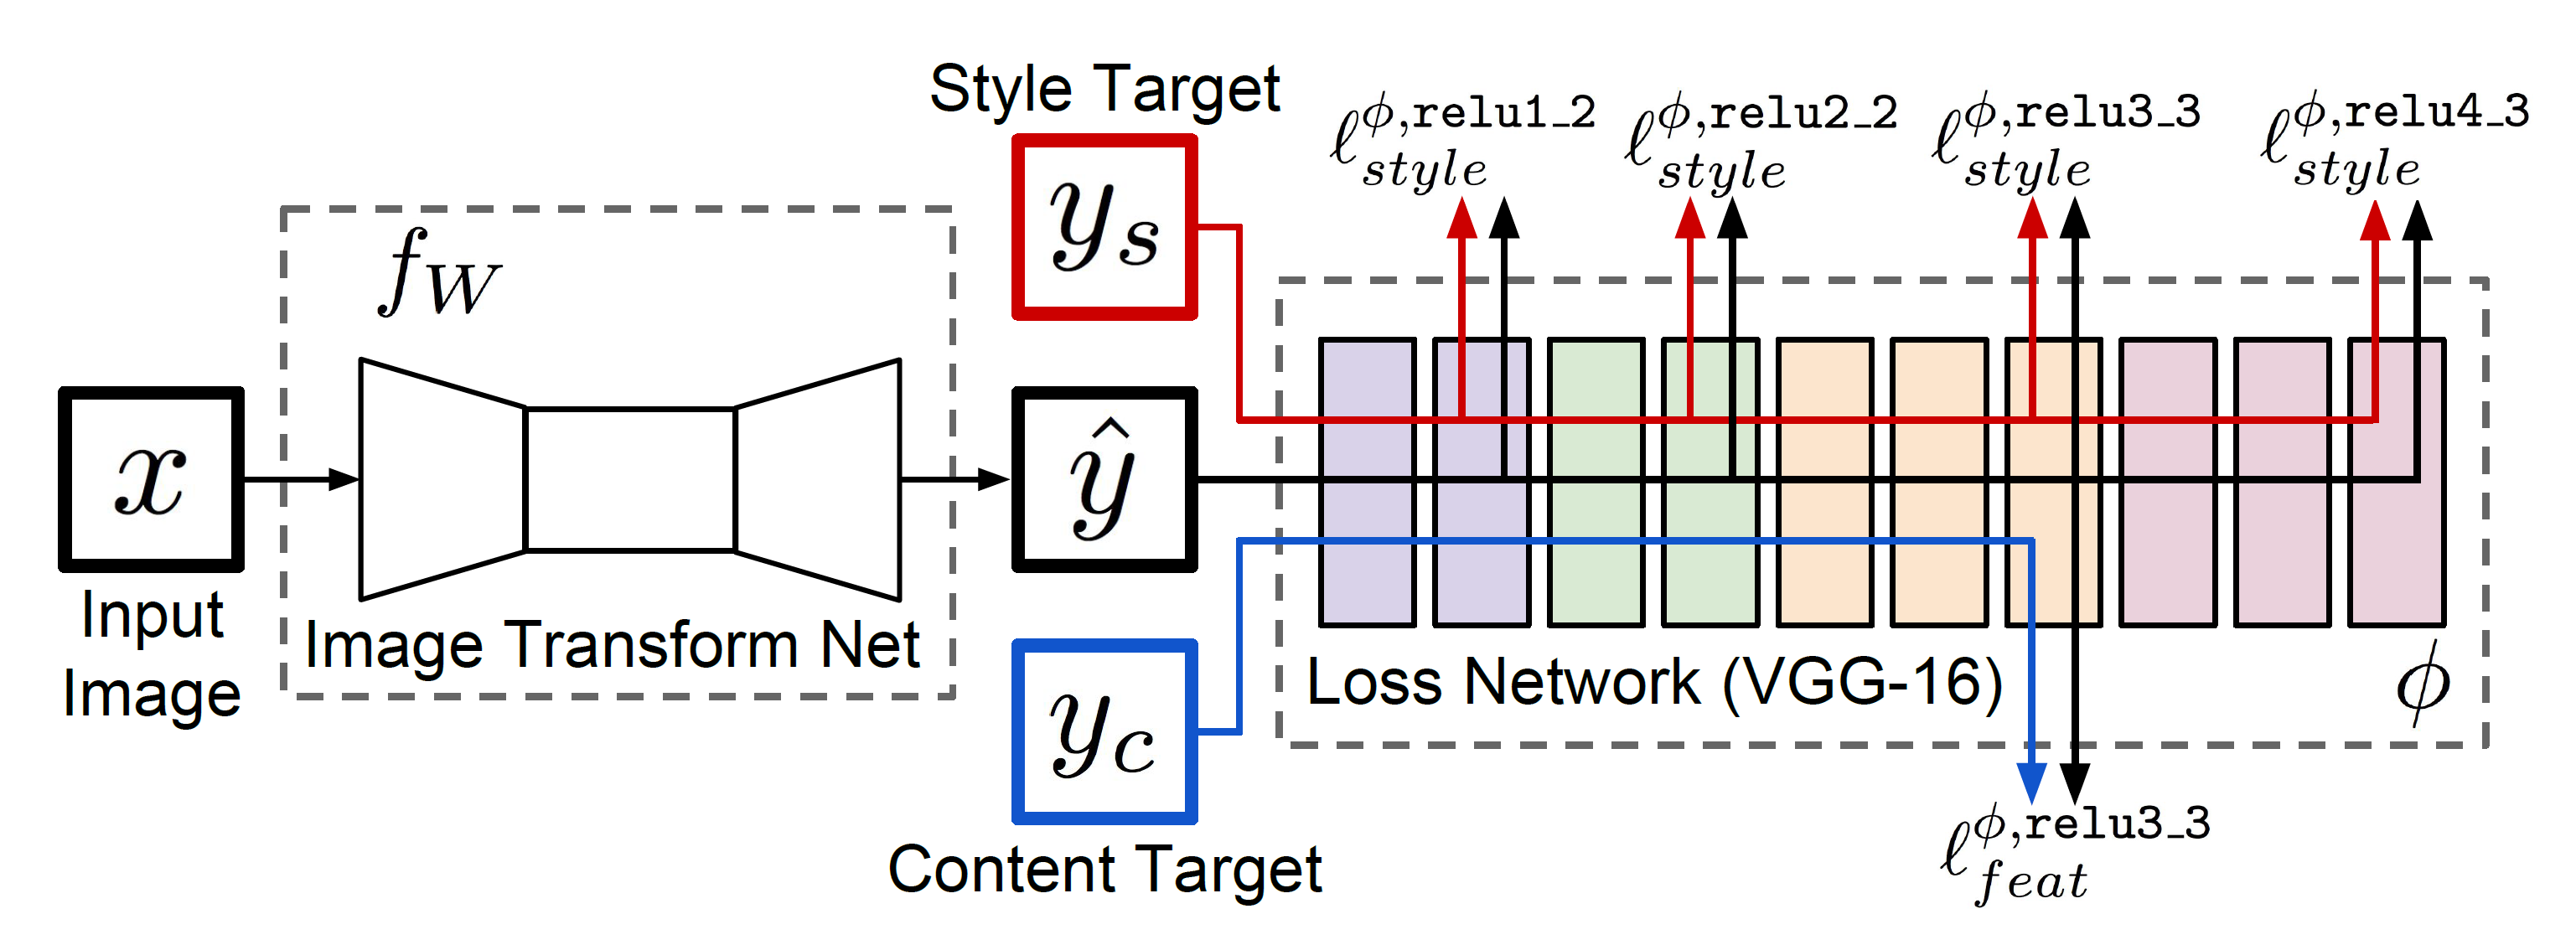
\includegraphics[width=\textwidth]{style_transfer_generator_network_johnson}%
	\caption{
		An image transformation network by Johnson et al. \cite{Johnson2016}.
		The image transform network (left) is the only one that changes.
		A loss network (right) is used to define perceptual loss functions.
	}
	\label{fig:style_transfer_generator_network_johnson}
\end{figure}
\begin{figure}
	\centering
	\subcaptionbox{Content Image \label{fig:style_transfer_ulyanov_content}}{%
		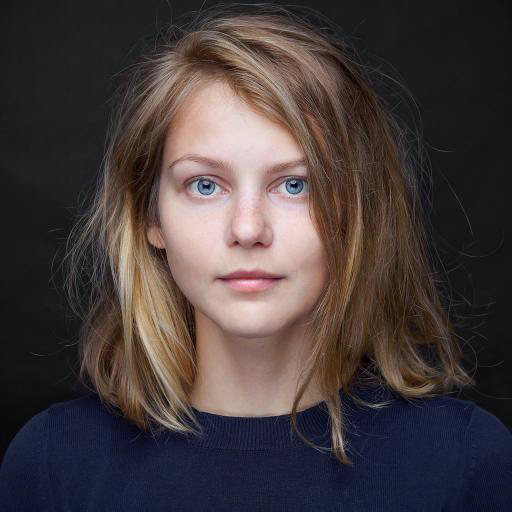
\includegraphics[width=0.2\textwidth]{style_transfer_ulyanov_content}%
	}
	\subcaptionbox{Style Image \label{fig:style_transfer_ulyanov_style}}{%
		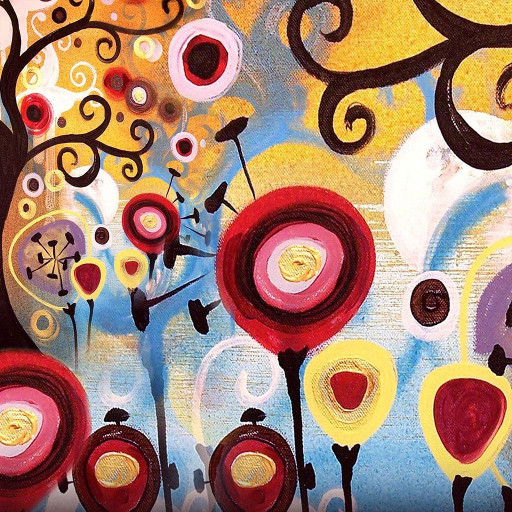
\includegraphics[width=0.2\textwidth]{style_transfer_ulyanov_style}%
	}
	\subcaptionbox{StyleNet with \gls{BN} \label{fig:style_transfer_ulyanov_BN}}{%
		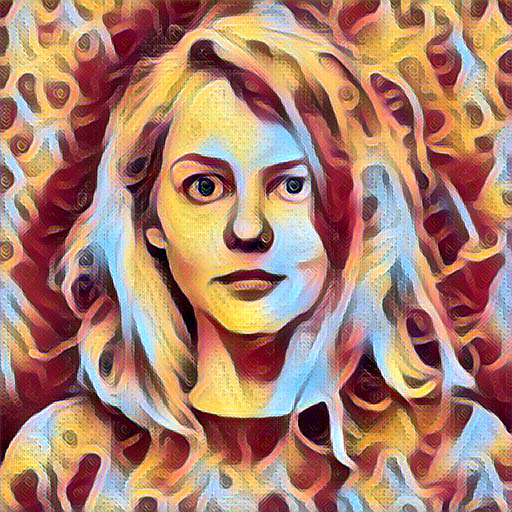
\includegraphics[width=0.2\textwidth]{style_transfer_ulyanov_BN}%
	}
	\subcaptionbox{StyleNet with \gls{IN} \label{fig:style_transfer_ulyanov_IN}}{%
		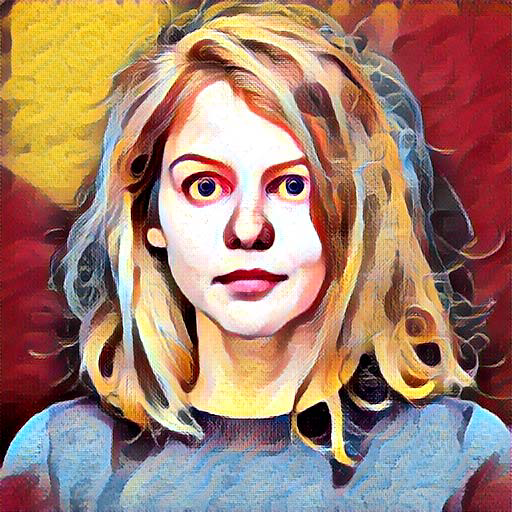
\includegraphics[width=0.2\textwidth]{style_transfer_ulyanov_IN}%
	}
	\caption{A comparison between (c) \gls{BN} and (d) \gls{IN}.\cite{Ulyanov2017}}
	\label{fig:style_transfer_ulyanov_BN_IN_comparison}
\end{figure}
\begin{figure}
	\centering
	\subcaptionbox{Content Image}[0.19\textwidth]{
		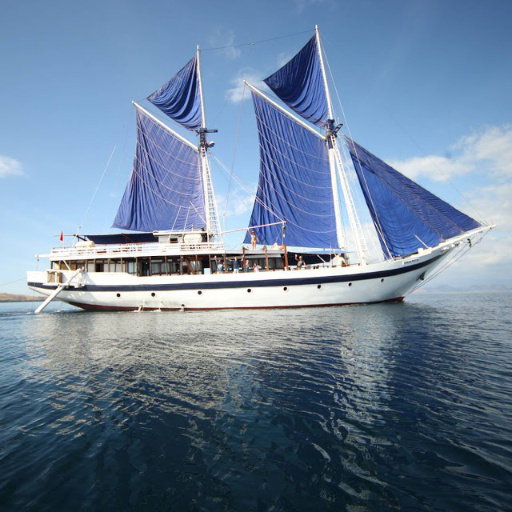
\includegraphics[width=0.19\textwidth]{style_transfer_content_a}\\
		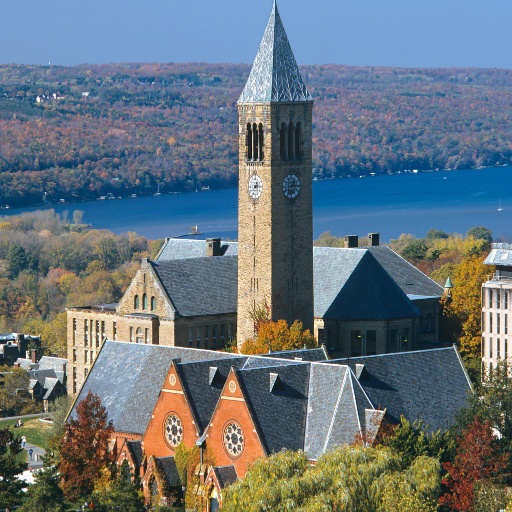
\includegraphics[width=0.19\textwidth]{style_transfer_content_b}\\
		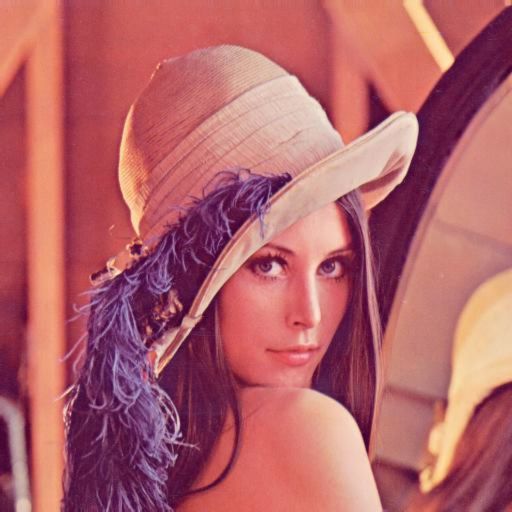
\includegraphics[width=0.19\textwidth]{style_transfer_content_c}\\
		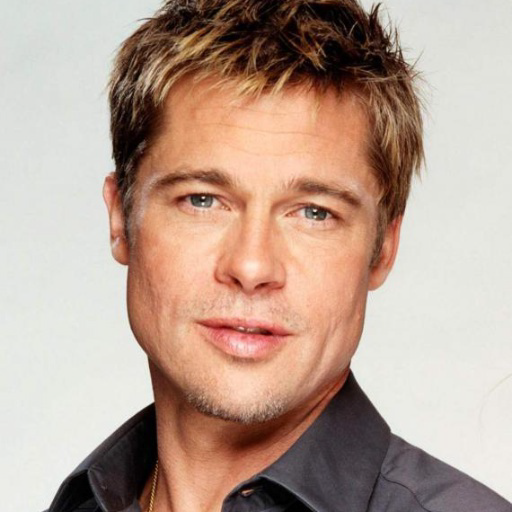
\includegraphics[width=0.19\textwidth]{style_transfer_content_d}\\
		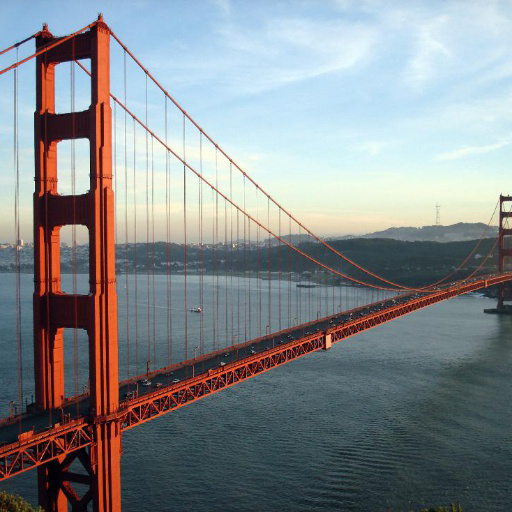
\includegraphics[width=0.19\textwidth]{style_transfer_content_e}\\
	}
	\subcaptionbox{Style Image}[0.19\textwidth]{
		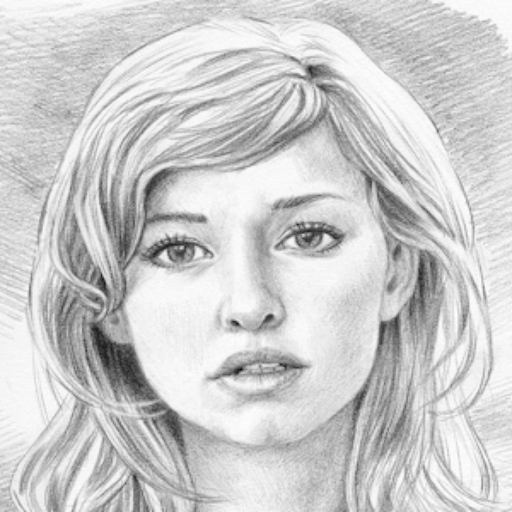
\includegraphics[width=0.19\textwidth]{style_transfer_style_a}\\
		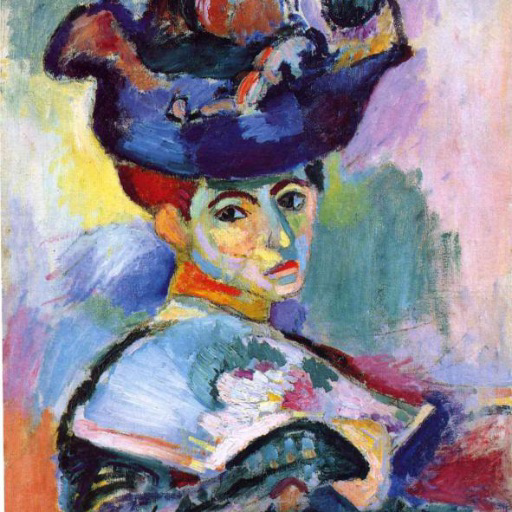
\includegraphics[width=0.19\textwidth]{style_transfer_style_b}\\
		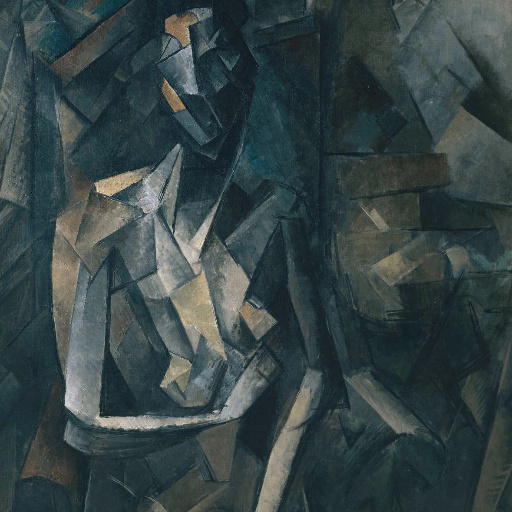
\includegraphics[width=0.19\textwidth]{style_transfer_style_c}\\
		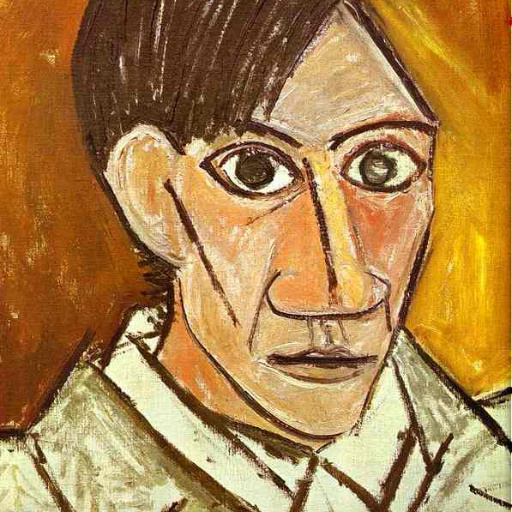
\includegraphics[width=0.19\textwidth]{style_transfer_style_d}\\
		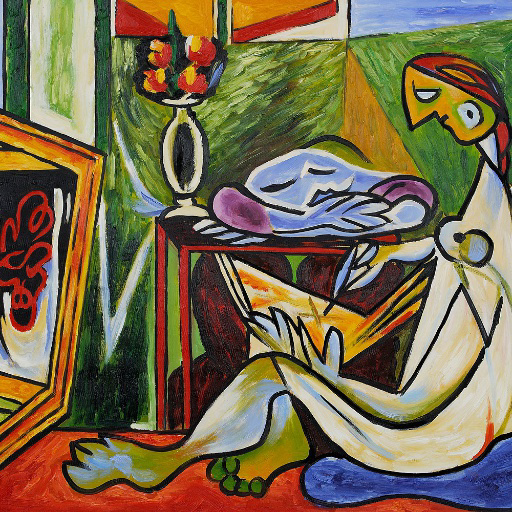
\includegraphics[width=0.19\textwidth]{style_transfer_style_e}\\
	}
	\subcaptionbox{Huang et al.}[0.19\textwidth]{
		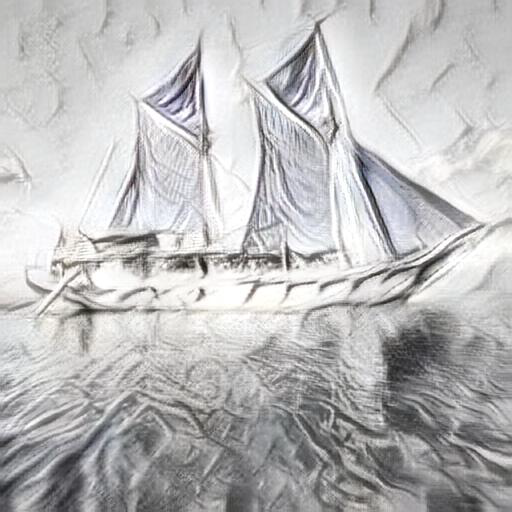
\includegraphics[width=0.19\textwidth]{style_transfer_huang_a}\\
		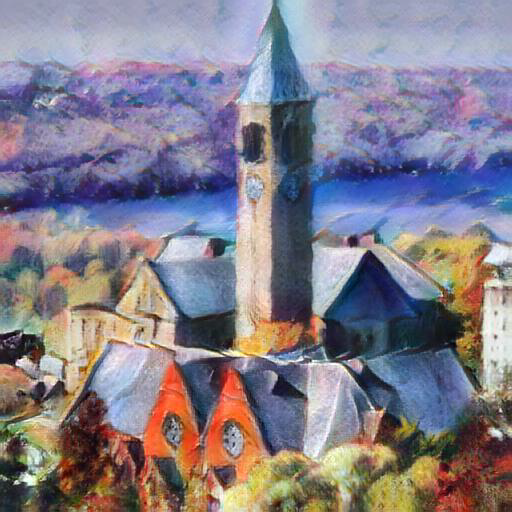
\includegraphics[width=0.19\textwidth]{style_transfer_huang_b}\\
		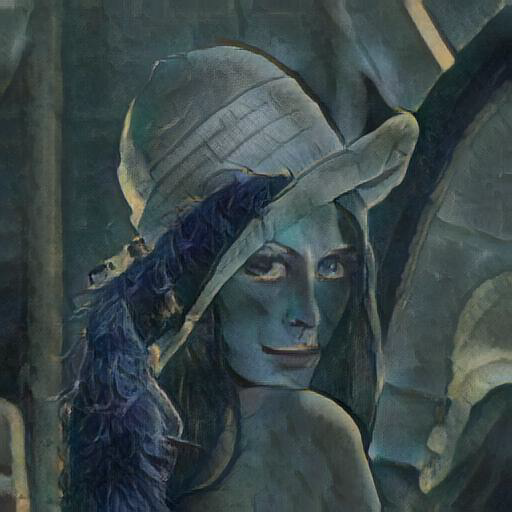
\includegraphics[width=0.19\textwidth]{style_transfer_huang_c}\\
		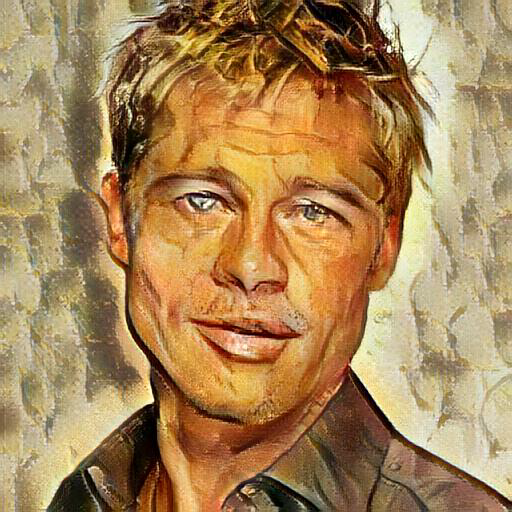
\includegraphics[width=0.19\textwidth]{style_transfer_huang_d}\\
		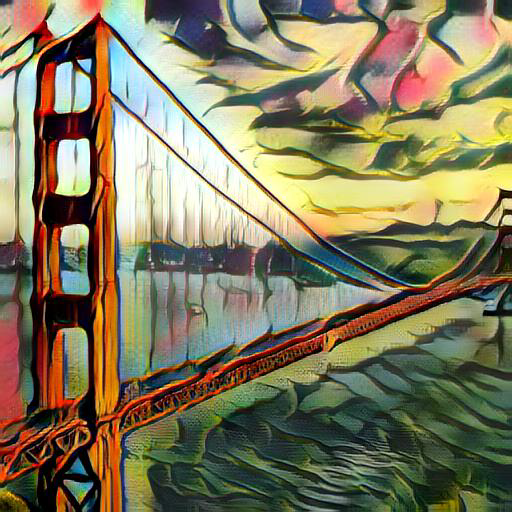
\includegraphics[width=0.19\textwidth]{style_transfer_huang_e}\\
	}
	\subcaptionbox{Ulyanov et al.}[0.19\textwidth]{
		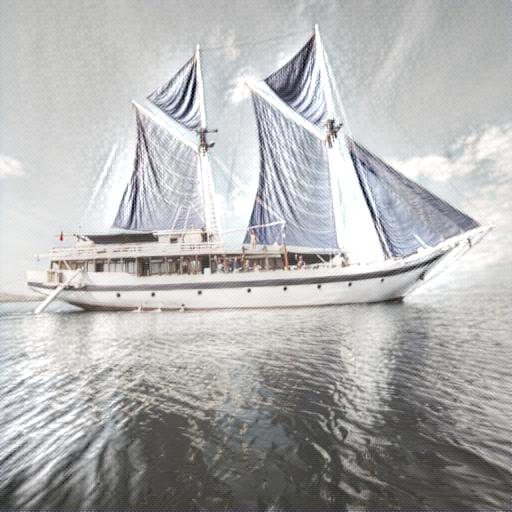
\includegraphics[width=0.19\textwidth]{style_transfer_ulyanov_a}\\
		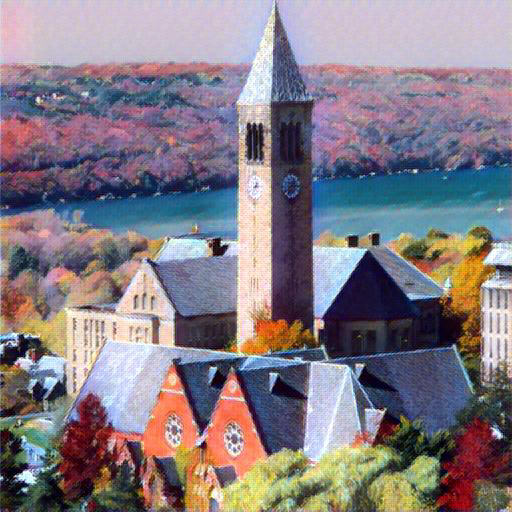
\includegraphics[width=0.19\textwidth]{style_transfer_ulyanov_b}\\
		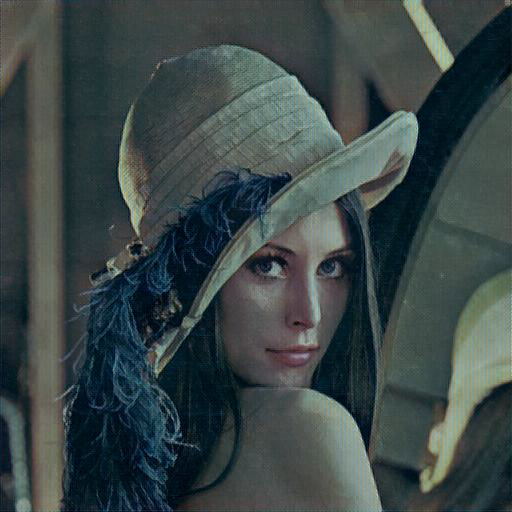
\includegraphics[width=0.19\textwidth]{style_transfer_ulyanov_c}\\
		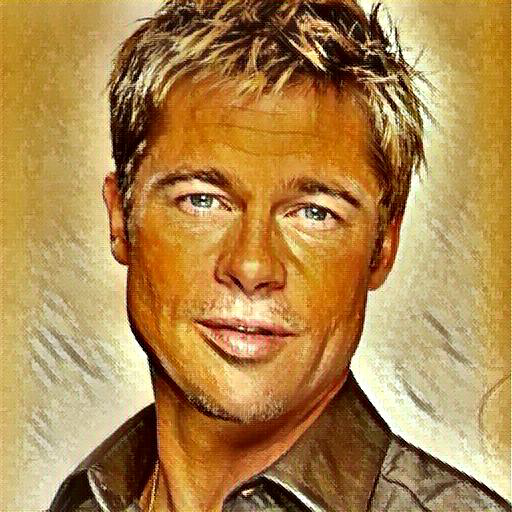
\includegraphics[width=0.19\textwidth]{style_transfer_ulyanov_d}\\
		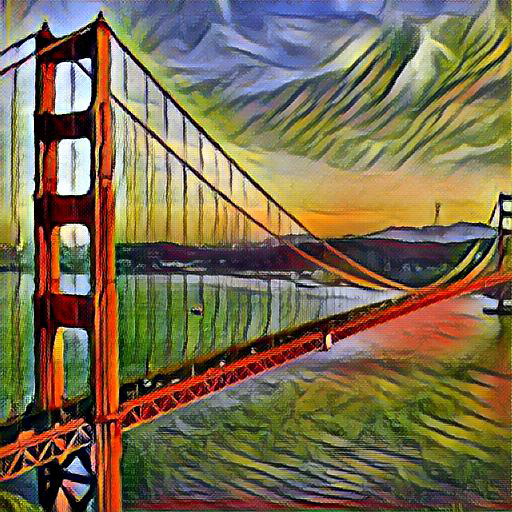
\includegraphics[width=0.19\textwidth]{style_transfer_ulyanov_e}\\
	}
	\subcaptionbox{Gatys et al.}[0.19\textwidth]{
		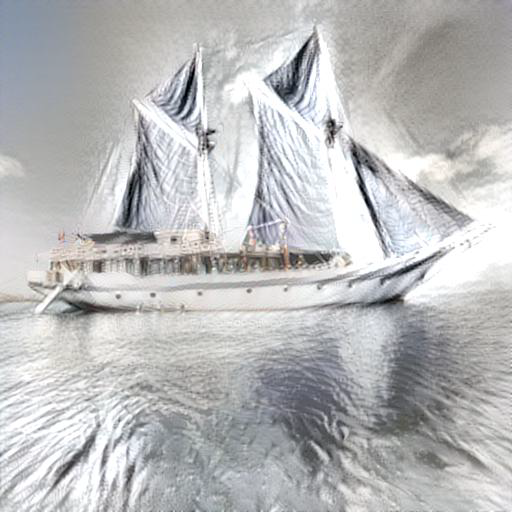
\includegraphics[width=0.19\textwidth]{style_transfer_gatys_a}\\
		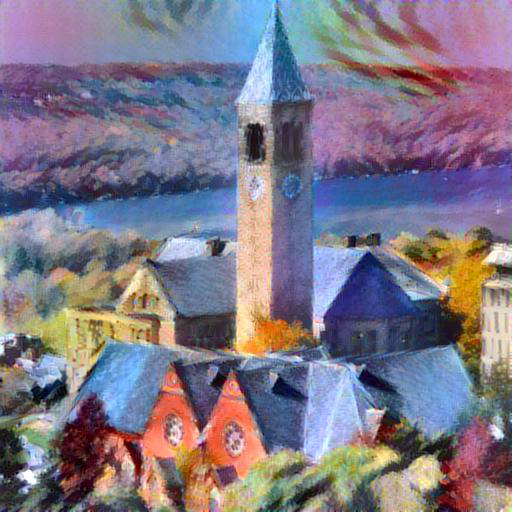
\includegraphics[width=0.19\textwidth]{style_transfer_gatys_b}\\
		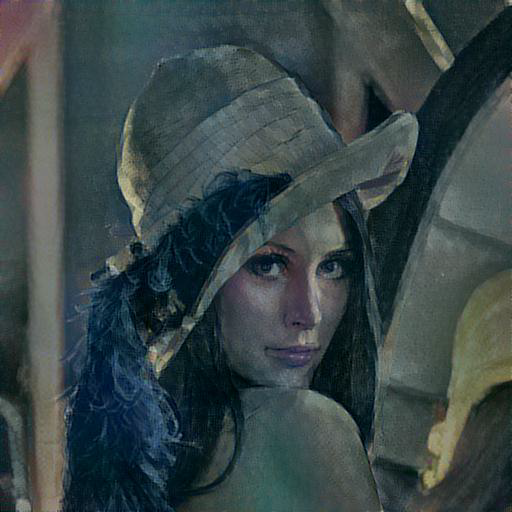
\includegraphics[width=0.19\textwidth]{style_transfer_gatys_c}\\
		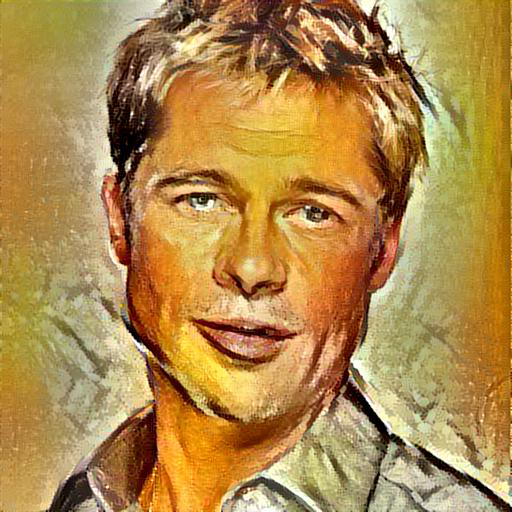
\includegraphics[width=0.19\textwidth]{style_transfer_gatys_d}\\
		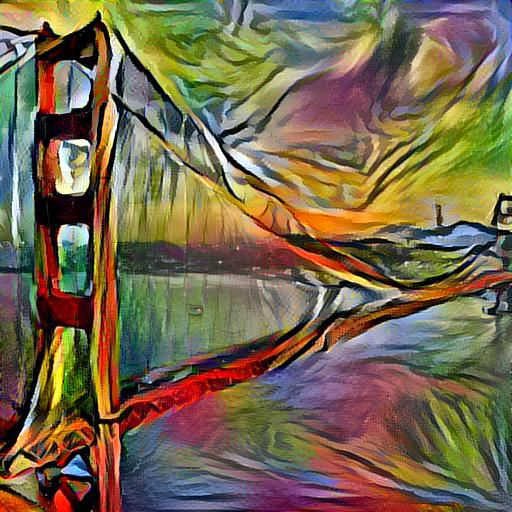
\includegraphics[width=0.19\textwidth]{style_transfer_gatys_e}\\
	}
	\caption{A comparison between different style transfers where the style was not seen during training.}
	\label{fig:style_transfer_unseen_style}
\end{figure}
\begin{figure}
	\centering
	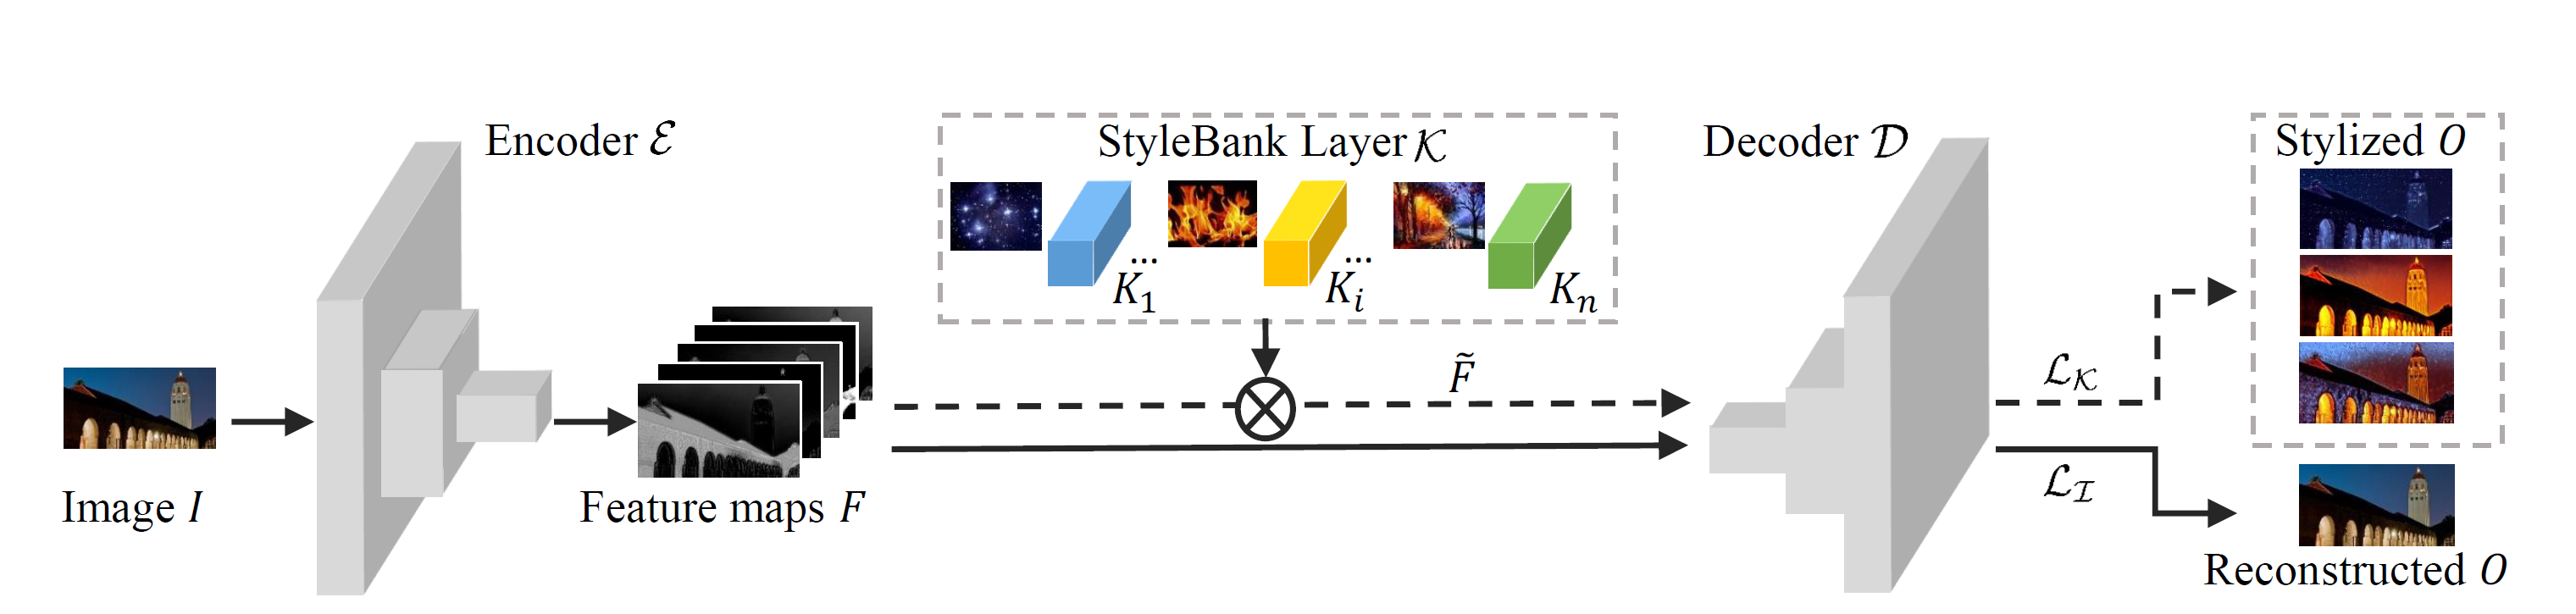
\includegraphics[width=\textwidth]{style_transfer_algorithm_stylebank}%
	\caption{
		The stylebank network by Chen et al. \cite{Chen2017}.
	}
	\label{fig:style_transfer_algorithm_stylebank}
\end{figure}
\begin{figure}
	\centering
	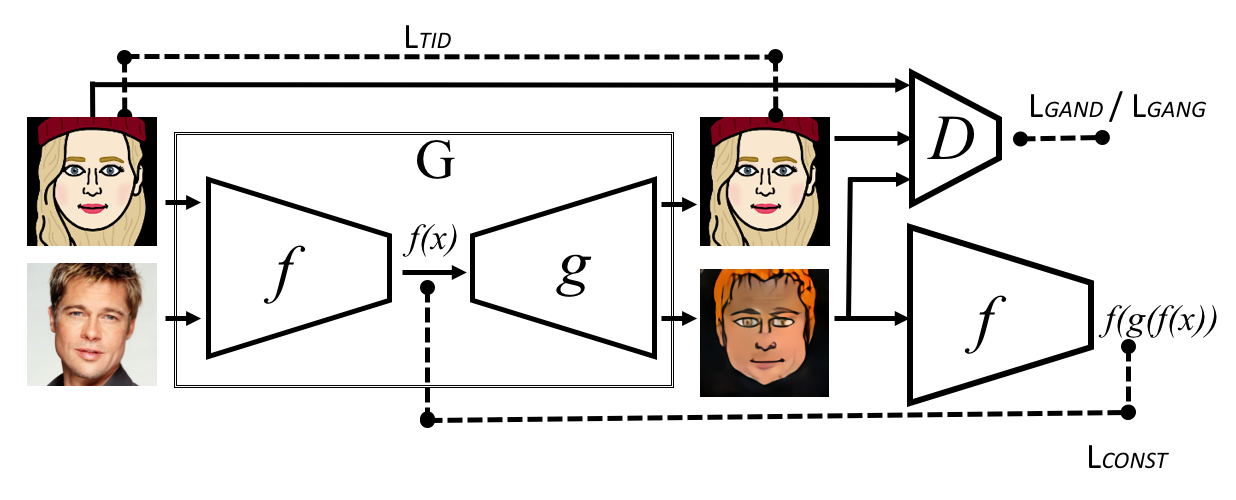
\includegraphics[width=\textwidth]{style_transfer_algorithm_taigman}%
	\caption{
		The domain transfer network by Taigman et al. \cite{Taigman2016}.
	}
	\label{fig:style_transfer_algorithm_taigman}
\end{figure}
\begin{figure}
	\centering
	\subcaptionbox{As illustrated by Zhu et al. \cite{Zhu2017}. \label{fig:style_transfer_algorithm_cyclegan}}{%
		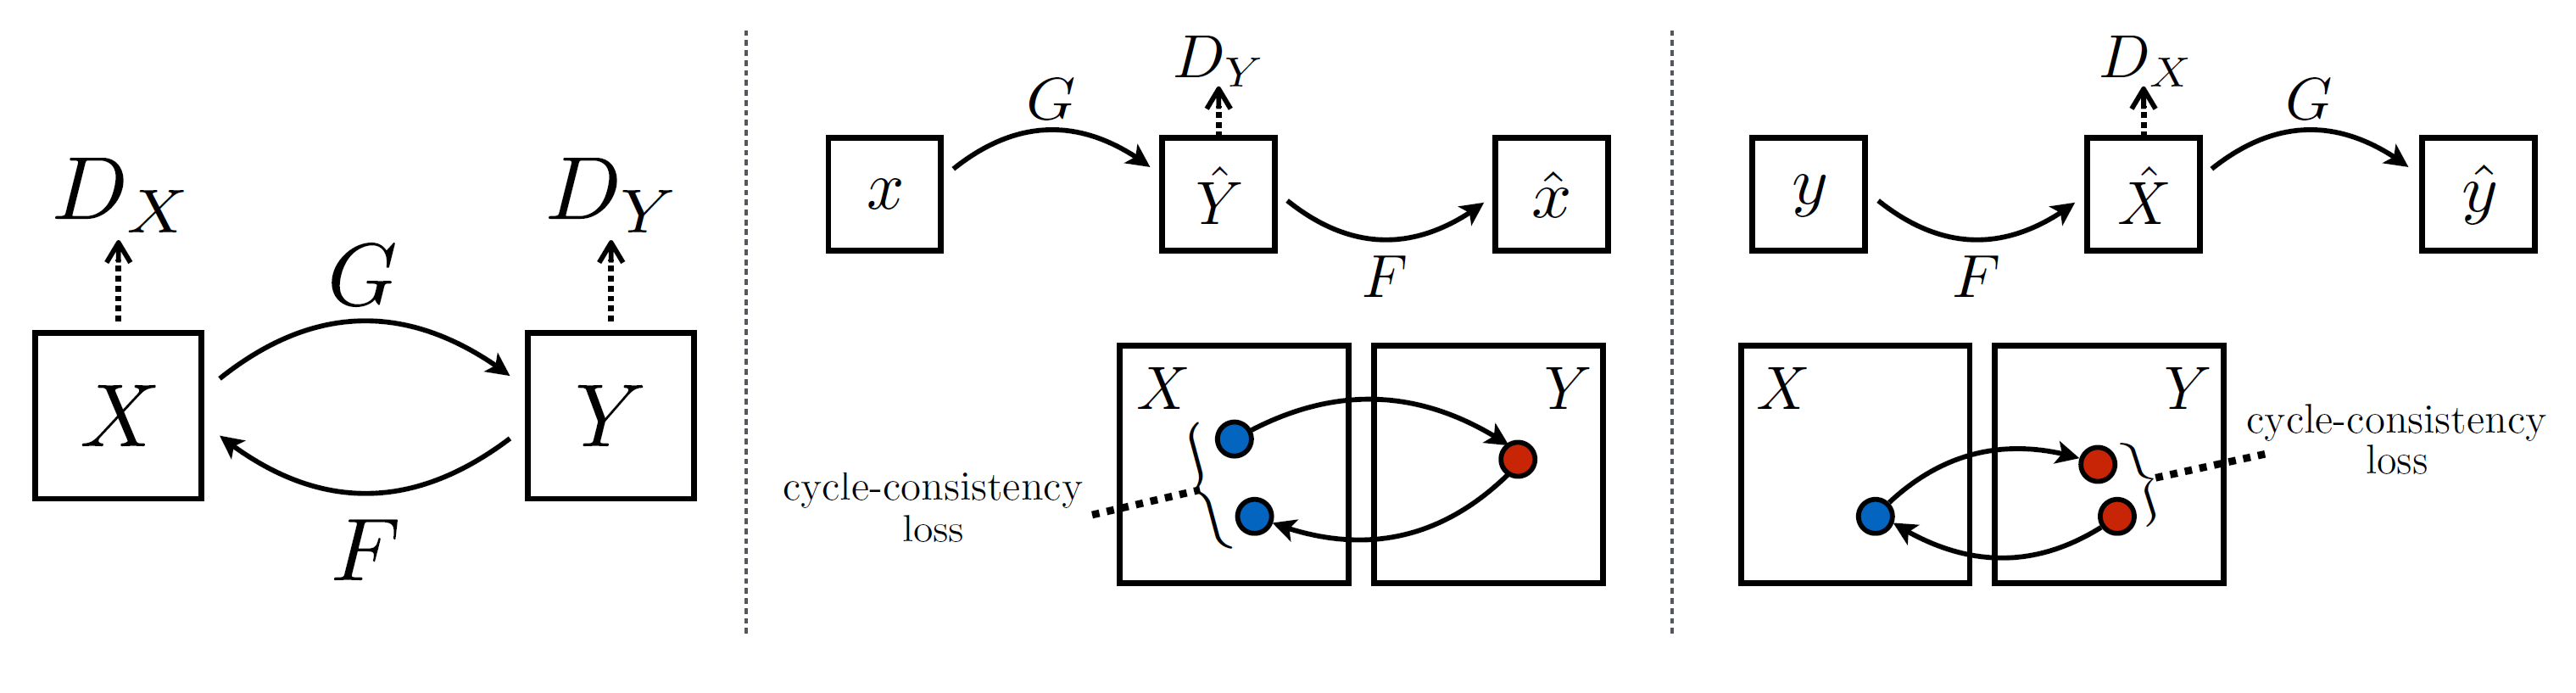
\includegraphics[width=\textwidth]{style_transfer_algorithm_cyclegan}%
	}
	\subcaptionbox{As illustrated by Kim et al. \cite{Kim2017}. \label{fig:style_transfer_algorithm_discogan}}{%
		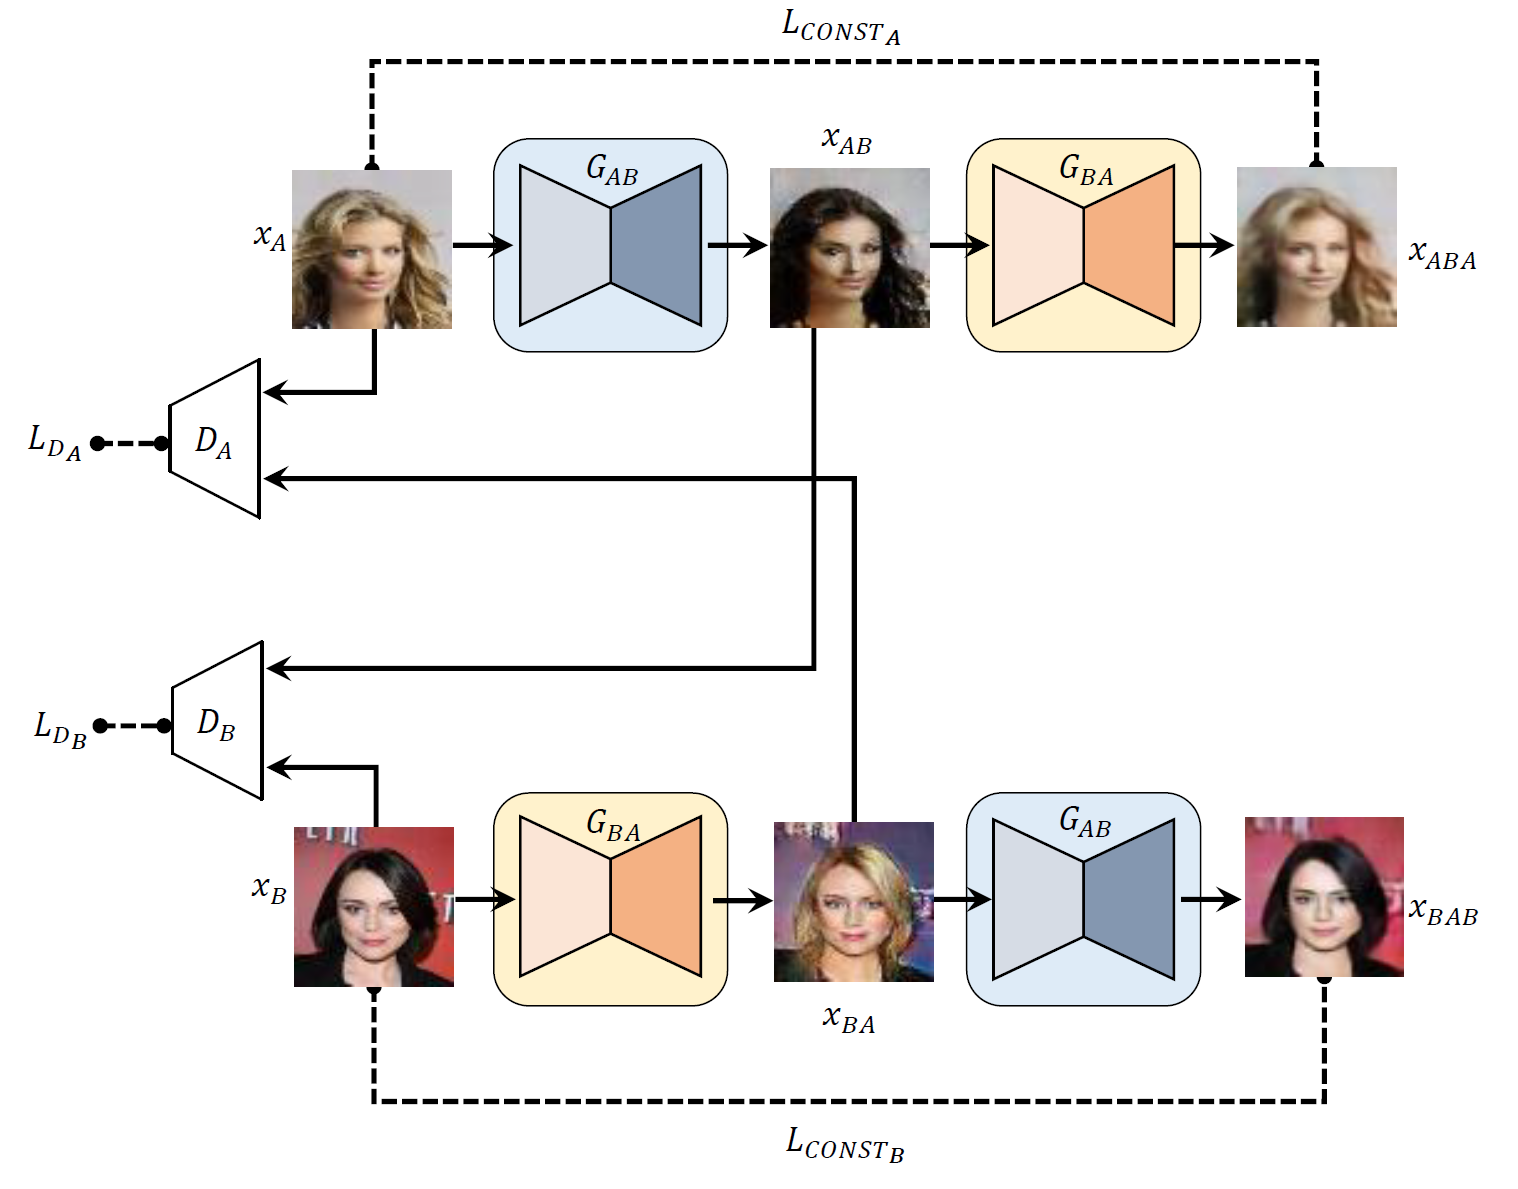
\includegraphics[width=\textwidth]{style_transfer_algorithm_discogan}%
	}
	
	\caption{
		The cycle-consistent network.
	}
	\label{fig:style_transfer_cyclegan}
\end{figure}
\begin{figure}
	\centering
	\includegraphics[width=\textwidth]{style_transfer_algorithm_unit}%
	\caption{
		(a) The shared latent space assumption.
		(b) The unsupervised image-to-image translation network by Liu et al. \cite{Liu2017}.
	}
	\label{fig:style_transfer_algorithm_unit}
\end{figure}
\label{sec:ist}